\documentclass[chaparabic,mmi,ms,12pt,single]{metu} 
\usepackage{appendix}
\usepackage{longtable}
\usepackage[pdftex]{hyperref}
\usepackage[all]{hypcap}
\usepackage{todonotes}
\graphicspath{ {./images/} }
\usepackage[figuresright]{rotating}
\usepackage{xy} 
\usepackage{booktabs}
\usepackage{pifont}
\usepackage{color}
\usepackage{listings}
\usepackage{pdfpages}
\usepackage{array}
\usepackage{algorithm}
\usepackage{algorithmic}
\usepackage{float}
\usepackage{caption}
\usepackage{lastpage}
\usepackage{afterpage}
\usepackage{lipsum}
\usepackage{adjustbox}
\usepackage{rotating}
\usepackage{pdflscape}
\usepackage{hypcap}
\usepackage{threeparttable}

\usepackage{graphicx}
\usepackage{tabularx}
\usepackage{amsmath,amssymb} % define this before the line numbering.
% \usepackage{ruler}
\usepackage{color}
% \usepackage{cite}
% \usepackage[utf8x]{inputenc}
% \usepackage{footnote}
% \makesavenoteenv{tabular}
% \makesavenoteenv{table}

\renewcommand{\sectionautorefname}{\S}
\renewcommand{\subsectionautorefname}{\S}

\newcommand{\norm}[1]{\left\lVert#1\right\rVert}

\captionsetup{belowskip=12pt,aboveskip=8pt}
\newcommand{\tab}{\hspace*{2em}}
\DeclareGraphicsExtensions{.pdf,.png,.jpg}
\DeclareCaptionLabelFormat{continued}{#1~#2 (Continued)}

\usepackage{amsmath}
\usepackage{siunitx}
\usepackage{textcomp}
\usepackage{subcaption}


\usepackage{tikz}
\usepackage{mathtools}
\usepackage{rotating}
%\PassOptionsToPackage{figuresright}{rotating}

\DeclarePairedDelimiter\ceil{\lceil}{\rceil}
\DeclarePairedDelimiter\floor{\lfloor}{\rfloor}
\usepackage{multirow}
\usepackage{hvfloat}

\newcommand{\EA}[1]{\textcolor{red}{[EA: #1]}}

% Name and Surname
\author{Aytekin Erdogan} % Change this
% Thesis Title English and Turkish
\title{A Transformer-Based Approach for Fusing Infrared and Visible Band Images} % Change this
\turkishtitle{Kızılötesi ve Görünür Bant Görüntülerin Birleştirilmesi İçin Transformer Tabanlı Bir Yaklaşım} % Change this

\date{August 2023} % Change this

 
% prof : Prof. Dr.
% assocprof : Assoc. Prof. Dr.
% assistprof : Assist. Prof. Dr.
% dr : Dr.
%
% Director of Institute
\director[prof]{ Banu GÜNEL KILIÇ} % Change this
% Head of Department
\headofdept[assocprof]{Elif SÜRER} % Change this
%
% Supervisor : English and Turkish
\supervisor[assocprof]{Elif SÜRER} % Change this
% \turkishsupervisor{  } %if you will hard-code the academic title
%
% Affiliation of Supervisor in English and possibly in Turkish
\departmentofsupervisor{Modeling and Simulation, METU} % Change this

\cosupervisor[assocprof]{Erdem AKAGÜNDÜZ} % Change this
\departmentofcosupervisor{Modeling and Simulation, METU} % Change this
%
% Committee Members
% In general members are sorted according to their academic titles
%
% Proffesors (1)
% Associate Professors (2)
% Assistant Professors (3)
% Other (4)
% 
% IMPORTANT:  All affiliatons should fit in a single line
% If affiliation line is broken into two lines you should shorten the affiliation by using 
% abbrevations or any other means
%
% First committee member should be the chair of examining committee
% Typically the chair is one of the highest ranked committee members
% Ask your supervisor if you are not sure
\committeememberi[prof]{Alptekin TEMİZEL} % Change this
\affiliationi{Modeling and Simulation, METU} % Change this
% Second committee member is always your supervisor
\committeememberii[assocprof]{Elif SÜRER} % Change this
\affiliationii{Modeling and Simulation, METU} % Change this
% If you are an M.Sc. student and your Co-Supervisor is in your 
% examination committee, then third committee member is always your co-supervisor
%
% IMPORTANT: If you are Ph.D. student your co-supervisor can not be in your 
% examination committee.

% \def\@proftitlename{Prof. Dr.}\def\@tproftitlename{Prof. Dr.}
% \def\@assocproftitlename{Assoc. Prof. Dr.}\def\@tassocproftitlename{Doç. Dr.}
% \def\@assistproftitlename{Assist. Prof. Dr.}\def\@tassistproftitlename{Yrd. Doç. Dr.}
% \def\@drtitlename{Dr.}\def\@tdrtitlename{Dr.}

\committeememberiii[assocprof]{İrem ÜLKÜ} % Change this
\affiliationiii{Computer Engineering Department, Ankara University} % Change this
% % Fourth committee member
% \committeememberiv[assistprof]{Committee Member 4} % Change this
% \affiliationiv{Department, School} % Change this
% % Fifth committee member
% \committeememberv[assistprof]{Committee Member 5} % Change this
% \affiliationv{Department, School} % Change this
%
% Keywords : English & Turkish, Comma seperated
\keywords{Image Fusion, Visual Infrared Image Fusion, Transformer Based Image Fusion, Structural Similarity Metric} % Change this
\anahtarklm{Görüntü Füzyonu, Görsel Kızılötesi Görüntü Füzyonu, Transformer Tabanlı Görüntü Füzyonu, Yapısal Benzerlik Ölçütü.} % Change this
%
% Abstract in English
%
\abstract{
  Image fusion is a process where images obtained from different sensors are combined to generate a single image that benefits from complementary information. Recently, there has been a growing interest in image fusion, which involves fusing images from diverse sensors to produce an enhanced image. Although deep learning methods have been widely employed in state-of-the-art techniques to extract meaningful features for image fusion, these methods primarily focus on integrating local features while disregarding the broader context within the image. To overcome this limitation, Transformer-based models have emerged as a promising solution, aiming to capture general context dependencies through attention mechanisms. Inspired by this, we propose a novel image fusion approach that incorporates a transformer-based multi-scale fusion strategy, effectively considering both local and general context information, thus enhancing the overall fusion process. Our proposed method follows a two-stage training approach, where an auto-encoder is initially trained to extract deep features at multiple scales. Subsequently, the multi-scale features are fused using a combination of Convolutional Neural Networks (CNNs) and Transformers. The CNNs are utilized to capture local features, while the Transformer handles the integration of general context features. Notably, in contrast to similar methods, we propose novel loss functions to address the challenges associated with defining a loss function when ground truth for fusion is absent. Through extensive experiments on various benchmark datasets, our proposed method, along with the novel loss function definition, demonstrates superior performance compared to other competitive fusion algorithms. Overall, this thesis presents significant advancements in image fusion techniques, offering innovative approaches and contributing to the state-of-the-art in this field.
} % Change this
%
% Turkish Abstract
%
\oz{
  Görüntü füzyonu, farklı sensörlerden elde edilen görüntülerin birleştirilerek tamamlayıcı bilgilerden yararlanan tek bir görüntü oluşturulması sürecidir. Son zamanlarda, farklı sensörlerden elde edilen görüntülerin birleştirilerek geliştirilmiş bir görüntü elde etme konusunda büyük bir ilgi artışı yaşanmaktadır. Derin öğrenme yöntemleri, görüntü füzyonu için anlamlı özelliklerin çıkarılmasında yaygın olarak kullanılmaktadır; ancak bu yöntemler genellikle yerel özelliklerin entegrasyonuna odaklanırken görüntünün daha geniş bağlamını dikkate almamaktadır. Bu kısıtlamayı aşmak için Transformer tabanlı modeller, dikkat mekanizmaları aracılığıyla genel bağlamlı bağımlılıkları yakalamayı hedefleyen umut vaat eden bir çözüm olarak ortaya çıkmıştır. Bu doğrultuda, yerel ve genel bağlam bilgisini etkili bir şekilde dikkate alan bir transformer tabanlı çok ölçekli füzyon stratejisi içeren yeni bir görüntü füzyon yaklaşımı önermekteyiz. Önerdiğimiz yöntem, ilk aşamada bir otokodlayıcı ile çok ölçekli derin özelliklerin çıkarılmasını sağlayan iki aşamalı bir eğitim yaklaşımını takip etmektedir. Ardından, çok ölçekli özellikler, Konvolüsyonel Sinir Ağları (CNN'ler) ve Transformer'ların bir kombinasyonu kullanılarak birleştirilmektedir. CNN'ler yerel özellikleri yakalamak için kullanılırken, Transformer genel bağlam özelliklerini entegre etmekten sorumludur. Benzer yöntemlere kıyasla, füzyon için gerçek değeri olmayan bir kayıp fonksiyonu tanımlama zorluklarını ele almak için yeni kayıp fonksiyonları önermekteyiz. Çeşitli benchmark veri kümeleri üzerinde yapılan kapsamlı deneylerle, önerilen yöntemimiz ve yeni kayıp fonksiyonu tanımı, diğer rekabetçi füzyon algoritmalarına kıyasla üstün performans sergilemektedir. Genel olarak, bu tez, görüntü füzyon tekniklerinde önemli ilerlemeler sunmakta, yenilikçi yaklaşımlar sunmakta ve bu alandaki en son teknolojiye katkıda bulunmaktadır.
} % Change this
%
% Dedications
\dedication{To those noble souls who, with selfless ardor, dedicate their entire lives for the betterment of humanity's plight} % Change this
%
%
% Acknowledgements   
\acknowledgments{
I want to express my deep gratitude to the remarkable individuals and organizations whose unwavering support made this thesis possible.

First and foremost, I want to thank the entire academic community at \textbf{Middle East Technical University}, especially my thesis advisors, \textbf{Assoc. Prof. Erdem Akagündüz} and  \textbf{Assoc. Prof. Elif Sürer}, for their invaluable guidance and insightful contributions to this research.

With utmost gratitude, I acknowledge \textbf{The Scientific and Technological Research Council of Turkey (TUBITAK)} for granting me the esteemed 2210A - Domestic Graduate Scholarship, which has been instrumental in funding this research endeavor. 

I am also thankful to the \textbf{Raventech Inc} for their collaboration, providing access to their computational resources that significantly elevated the quality and efficiency of this study.

In addition, I must mention the \textbf{BlueJay Coffee House}, where I found a haven during this research journey. Their delicious coffee made from unique beans from around the world kept me energized and focused.

% To an \textbf{anonymous friend}, I owe my gratitude for unknowingly providing comfort and peace through their friendly smile and presence during this demanding process.

Lastly, To my \textbf{family and friends}, I am deeply indebted for their unwavering encouragement and support in every step of this academic pursuit.

With heartfelt appreciation, I recognize the profound impact each of you has had on this academic journey, and I am truly grateful for your invaluable contributions.
} % Change this

%
% End of Personal and Introductory Information
%%%%%%%%%%%%%%%%%%%%%%%%%%%%%%%%%5
\begin{document}
% Preliminaries
\begin{preliminaries}
% If you are willing to use any custom stuff before Chapters, put it here
% Such as List of Abbreviations
% Check the abbreviations.tex for a template list of abbreviations

\input{abbreviations.tex}
% End of Preliminaries
\end{preliminaries}
%   
% Latex content Goes Here 
% 
%

\setlength{\parindent}{0em}
\setlength{\parskip}{10pt}

% You can add as many chapters
% Change this
\label{chp:introduction}
The intricate evolution of perception systems across species, from minuscule insects to towering apex predators, showcases nature's mastery. As humans delve into technological innovation, we've engineered mechanical eyes that not only emulate but at times exceed their biological counterparts. This intertwining of natural instincts and modern camera technology manifests a limitless realm of perception. Central to computer vision is the spectrum of light, which extends from the visible colors our eyes discern, around 400 to 700 nanometers, to realms beyond human sight, including the warmth of infrared and the energy of ultraviolet waves. While humans are limited to a segment of this spectrum, technology unlocks a wider expanse, particularly through both visible and infrared imagery, heralding a revolutionary phase in computer vision. Image fusion leverages multiple image sources, offering enhanced clarity and understanding, and is pivotal in contemporary computer vision. Specifically, Visual-Infrared Image Fusion (VIF) melds visible and infrared spectrums, proving transformative for applications like night vision and thermal imaging. This fusion augments perception in low-visibility conditions, benefiting sectors like the military and security. Various techniques, from traditional pixel and feature-level fusion to advanced learning methods such as CNN-based and transform-based fusion, are employed to effectively merge these images, amplifying situational comprehension across applications.

\subsection{Problem Definition}\label{sec:probdef}

While deep learning methods excel at extracting pertinent features for image fusion, their primary focus on local features often neglects the overarching context within the image, a concern raised by Li et al. (2021)\cite{li2021rfn}. Transformer-based models, employing attention mechanisms, offer a solution, capturing wider context dependencies to refine fusion outcomes.

A significant impediment in fusion techniques is crafting the appropriate loss function. Conventional methods rely heavily on the Structural Similarity Metric (SSIM) to ascertain similarity between the input visible band image and the fused output. This SSIM-centric approach has its limitations, given that its maximum value is only achieved when both images are identical. To address this, we suggest a novel loss function that places equal emphasis on congruence with both the visible band and infrared inputs. This dual-input consideration ensures optimal retention of essential information, bolstering the quality of the fusion.

In response to the pressing need for enhanced image fusion techniques, our research bifurcates into two pivotal studies. The primary study delves deep into innovating the loss function. Central to this exploration is the creation of a loss function that harmonizes the similarity between both visible and infrared inputs. Traditional methods often marginalize this aspect, leading to subpar fusion results. Our proposed function seeks to remedy this, fostering a more efficient and meaningful fusion process.

Through this structure, we aim to fully harness the potential of image fusion techniques, heralding not just advancements in current applications but also paving the way for future innovations.

\subsection{Research Questions and Hypotheses} \label{sec:researchquestions}

To gain a comprehensive understanding of the complexities surrounding image fusion, our research seeks to answer the following hypotheses, systematically divided into two studies based on their thematic focus:

\subsubsection{New Loss Function Proposal}

\begin{list}{}{}{}
    \item \textbf{Hypothesis 1}: The new loss function, which emphasizes the similarity between both the visible band input and the infrared image input, will result in more informative and meaningful fused images compared to using Structural Similarity Metric (SSIM) as the guiding criterion.
    \item \textbf{Hypothesis 2}: The proposed approach will surpass existing state-of-the-art image fusion methods in terms of visual quality, providing more detailed, sharper, and visually appealing fused images.
\end{list}

This structured presentation of research questions and hypotheses aims to provide a clear roadmap for our investigation. Through rigorous testing of these hypotheses, our ultimate goal is to validate or challenge them, leading to significant contributions to the field of image fusion. By systematically evaluating each hypothesis within the respective studies, we aim to draw conclusions that are both robust and comprehensive, thereby advancing the current state of knowledge within this domain.


\subsubsection{A Unique Transformer Based Fusion Strategy}

\begin{list}{}{}
    \item \textbf{Hypothesis 3}: The combination of Transformer-based models and the new loss function will significantly improve night vision enhancement, medical imaging, and surveillance tasks, allowing for better object detection, classification, and tracking in challenging lighting conditions.
    \item \textbf{Hypothesis 4}: The proposed transformer based approach will achieve a better balance between quantitative and qualitative performance in image fusion, overcoming the compromise between the two that is often observed in traditional deep learning methods.
    \item \textbf{Hypothesis 5}: The proposed approach will demonstrate computational efficiency, making it suitable for real-time applications, such as video surveillance and live medical imaging, without sacrificing the quality of the fused images.
    \item \textbf{Hypothesis 6}: The limitations and challenges associated with implementing Transformer-based image fusion techniques can be mitigated through proper model tuning, regularization, and architecture adjustments, leading to improved overall performance.
\end{list}
\label{chp:RelatedWork}

The domain of RGB and infrared image fusion has been a focal point of substantial research, witnessing a plethora of innovative methods from the early 1990s to the cutting-edge Transformer-based models. These techniques span categories like Traditional Fusion Algorithms, CNN, Autoencoder, GAN, and notably, Transformer-based approaches where attention mechanisms optimize the fusion. Within this vast spectrum, a key challenge is the limited availability of labeled datasets due to the inherent complexity of fusing RGB and IR images. As a result, our research navigates the unsupervised scenario, leveraging various Performance Evaluation and Benchmarking metrics to quantify the fusion results, offering insights into the strengths, limitations, and practical applications of each method. This chapter culminates in our exploration of Transformer-based algorithms, representing a comprehensive journey through RGB and IR image fusion techniques and challenges.

Image fusion algorithms can be classified based on factors like the use of learning methods versus hand-crafted steps, predefined loss functions, and the involvement of labeled datasets. While learning-based methods like CNN, GAN, Transformers, and Auto-encoders harness machine learning to understand input images, hand-crafted approaches involve manual feature design and fusion rules. The categorization extends to whether methods are end-to-end or require intermediary handcrafted steps. Furthermore, loss functions guide the training process, leading to classifications like self-supervised, supervised, or unsupervised based on the loss function. Labeled datasets, whether for training learning-based methods where ground-truth is known or for evaluating fusion algorithms, play a pivotal role. These considerations help researchers select the most apt image fusion algorithm tailored to their application requirements.

\subsubsection{Traditional Fusion Algorithms}
\label{sec:traditional}

Traditional image fusion algorithms, while extensively studied, come with inherent shortcomings, notably the presence of handcrafted steps leading to potentially suboptimal results and high time complexity in some cases. Sparse representation (SR) based methods, such as those by Bin et al \cite{bin2016efficient} and Zhang et al \cite{zhang2013dictionary}, are popular but are limited by requirements like dictionary learning, which increases their time complexity, and handcrafted steps affecting their generalizability. Multi-scale transformation (MST) based methods, exemplified by Hu et al \cite{hu2017adaptive} and others \cite{he2017infrared}, are effective at capturing image characteristics at varying scales but can lack generalizability in specific contexts. Low-rank representation (LRR) methods, like those from Liu et al \cite{liu2012robust}, excel in handling noise and image degradation, but may falter with complex textures or patterns. Ultimately, the efficacy of traditional fusion algorithms largely hinges on the chosen feature extraction method, necessitating careful consideration of the problem's specific demands before settling on a technique.

\subsection{Learning Based Algorithms for Image Fusion}

\subsubsection{CNN Based Algorithms}
Liu et al. were among the first to introduce a method for image fusion that utilizes CNN, focusing on the fusion of infrared and visible images \cite{liu2018infrared}. Their approach consisted of several steps, from preprocessing to feature extraction, fusion strategy, and reconstruction, achieving better fusion results than other state-of-the-art methods of the time. CNN-based methods are generally divided into supervised and unsupervised categories. While both utilize CNNs for feature extraction, supervised methods require labeled data, often leveraging techniques like data augmentation or transfer learning. Unsupservised methods, on the other hand, don't require labeled data, making them more flexible for real-world applications. Despite their success, there's room for improvement, especially in situations where input images have significant differences in factors like illumination or resolution.

\subsubsection{Autoencoder Based Algorithms}
Autoencoders, a type of neural network, have been widely used for tasks like dimensionality reduction and data compression. Within the domain of infrared visual image fusion, autoencoders are leveraged to extract features from source images in the encoder stage, while the decoder stage focuses on reconstructing the fused image. The training process involves two stages: firstly, training the autoencoder using source images without any fusion, followed by integrating the fusion step. Notable works in this area include DenseFuse \cite{li2019infrared} and studies by Raza et al. \cite{raza2020pfaf} and Fu et al. \cite{fu2021dual}, among others.

\subsubsection{GAN Based Algorithms}
Since their introduction by Goodfellow et al. \cite{goodfellow2014generative}, GANs have found diverse applications, including image fusion. The majority of GAN-based image fusion methods are unsupervised, focusing on the difference between the fused and source images. Innovations in this space include the use of multiple discriminators, as seen in methods introduced by Ma et al. \cite{ma2020ganmcc} and Xu et al. \cite{xu2019learning}, and the integration of attention mechanisms and residual connections for improved performance.

\subsubsection{Transformer Based Algorithms}
\label{sec:Transformer}

Transformers have risen as paramount tools in managing long-range dependencies in fields like natural language processing and computer vision \cite{dosovitskiy2020image, liu2021swin, liu2022mfst}. Their introduction into image fusion in 2021 revolutionized the domain, with several innovative methodologies emerging \cite{zhao2021dndt, rao2023tgfuse, li2022cgtf, tang2022ydtr, wang2022swinfuse, yang2023dglt, tang2023tccfusion}. 

Central to these methodologies is the self-attention mechanism, enhancing fusion outcomes by preserving essential details and efficiently blending features. For instance, VS et al. \cite{vs2022image} introduced a multiscale fusion strategy harnessing this architecture, while Zhao et al. \cite{zhao2021dndt} advanced a dual transformer approach. Noteworthy strategies also include the integration of transformers with traditional methods, as evidenced by Fu et al.\cite{fu2021ppt}, Wang et al. \cite{wang2022swinfuse}, and others.

Transformer-based VIF techniques predominantly operate unsupervised, leveraging loss functions from the comparison of fused and source images. While this eliminates the need for annotated data, it also complicates methodological evaluations due to the absence of a direct quality reference.

With increasing research into transformer-based image fusion, the focus remains on novel designs and methodologies, such as diverse transformer integrations in the fusion pipeline, transformer-CNN combinations, and the utilization of auxiliary information to enrich fusion processes.

\label{chp:b3}

In this chapter, we delve into the realm of infrared and visual band image fusion using transformers, offering a detailed account of our experimental setup and the rationale for our model selection that marries autoencoders with fusion transformers. The robustness of our research is grounded in the carefully curated datasets described in Section \ref{subsec:dataset}, which encompass diverse real-world scenarios and are tailored for compatibility with our fusion model. The infrastructure supporting our research, detailed in Section \ref{subsec:platform}, boasts state-of-the-art GPUs, enhancing our model's training and inference speeds. Our image fusion model's foundation, the autoencoder, is explored in Section \ref{subsec:aesel}, highlighting its capability to distill crucial features from both image bands, subsequently processed by our fusion transformer—a novel yet unclaimed pioneering approach in the field—described in Section \ref{subsec:fusion}. Our commitment to refining image fusion is further emphasized by our tailored loss functions, delineated in Sections \ref{subsec:aeloss} and \ref{subsec:fusionloss}, which play pivotal roles in our model's training to achieve superior fusion results. Through this exploration, we aspire to advance the horizons of multi-modal image processing, heralding advancements in areas like remote sensing and surveillance.
\subsection{Model Selection} \label{sec:model}

Image fusion, as discussed in Section \ref{sec:traditional}, is a complex problem that can be broken down into three distinct components: the feature extractor, feature fuser, and image reconstructor. The first part of the solution, the feature extractor, plays a crucial role in obtaining multilevel features from the input images. These extracted features are then passed on to the feature fuser, which constitutes the second part of the model. Here, the feature fuser's primary task is to identify complementary features from the previously obtained multilevel features and fuse them into a single set of feature maps for each level. These fused multilevel features serve as the foundation for reconstructing the final fused image, handled by the image reconstructor, which is the third and final part of the model.

Upon closer examination, it becomes evident that the feature extractor bears a resemblance to the encoder part of autoencoders, as discussed in Section \ref{sec:AE}. On the other hand, the image reconstructor can be likened to the decoder part of autoencoders. This analogy helps to conceptualize the flow of information within the model, and it emphasizes the importance of effectively extracting and fusing features to achieve a successful image fusion.

To implement the feature fuser, the model leverages a combination of Convolutional Neural Networks (CNNs) and transformers, as indicated in Section \ref{sec:CNN} and Section \ref{sec:Transformer}, respectively. CNNs are well-suited for local feature matching and combination, whereas transformers excel at handling global contextual information. By integrating these two components, the model aims to strike a balance between capturing intricate local details and grasping broader contextual relationships. This fusion of methodologies holds the potential to enhance the model's performance and produce more accurate image fusions.

\begin{figure}[htbp]
    \centering
    % \vspace{0.01cm}
    \begin{subfigure}[b]{\textwidth}
        % \centering
        \includegraphics[width=0.4\textwidth]{../01metu-msc-thesis/images/ch3/20230815all.drawio.pdf}
        \caption{Detailed Design of Model}
        \label{fig:ch3:highlevel}
    \end{subfigure}
    \vspace{0.01cm}
    \begin{subfigure}[b]{\textwidth}
        % \centering
        \includegraphics[width=0.4\textwidth]{../01metu-msc-thesis/images/ch3/20230815STAGE2.drawio.pdf}
        \caption{High-Level Algorithmic Detailed Design of Model}
        \label{fig:ch3:highlevel2}
    \end{subfigure}
    \caption{Design of Overall Model}
    \label{fig:ch3:rfnnest}
\end{figure}

Given the problem's complexity and the proposed model configuration, it is essential to conduct in-depth analyses of each aspect. Therefore, the subsequent sections, from \ref{subsec:aesel} to \ref{subsec:fusionloss}, delve into a comprehensive exploration of the model's inner workings, the datasets employed during experimentation, and the design of the loss function used to train the model. This deeper understanding will shed light on the model's capabilities and limitations, providing a solid foundation for testing and evaluating the proposed hypothesis.

\subsubsection{Stage 1: Autoencoder Selection} \label{subsec:aesel}

Training autoencoders presents a set of challenges that require careful consideration and effective solutions. One of the primary obstacles encountered is the vanishing or exploding gradients during backpropagation, which can hinder the convergence of the model. To overcome this, using activation functions like $ReLU$ and employing gradient clipping techniques can stabilize the training process. Another critical issue is overfitting, where the model becomes too specialized to the training data. Regularization methods such as $L1$ or $L2$ regularization and dropout can help prevent overfitting and improve generalization.

\begin{figure}[htbp]
    \centering
    \includegraphics[width=0.5\textwidth]{../01metu-msc-thesis/images/ch3/20230815stage1.drawio.pdf}
    \caption{Autoencoder High-Level Design}
    \label{fig:ch3:encoderhighlevel}
\end{figure}

Additionally, selecting the right dimension for the latent space is vital in autoencoders. A comprehensive hyperparameter search and evaluation using techniques like cross-validation can guide the choice of an appropriate latent space dimension. Moreover, traditional autoencoders might struggle with multimodal data, producing unimodal outputs.Data preprocessing also plays a crucial role in training autoencoders. Careful normalization, scaling, and augmentation techniques can improve the model's robustness and performance. However, dealing with large and deep autoencoder architectures can be computationally expensive. To address this issue, optimizing the model architecture, reducing the number of parameters, and utilizing hardware accelerators like GPUs or TPUs can significantly speed up training.

Despite their capabilities, autoencoders may produce learned features that lack human interpretability. Techniques like activation maximization and feature visualization can aid in understanding the representations learned by the model. Additionally, enforcing sparsity constraints in the encoder can encourage the extraction of more interpretable and compact features.

By addressing these challenges and applying appropriate solutions, autoencoders can become powerful tools for learning meaningful representations, enabling a wide range of applications in various domains. The combination of theoretical insights and practical strategies is essential for designing robust autoencoder architectures that can tackle complex real-world problems effectively.

\begin{list}{}{}
    \item \textbf{Vanishing or Exploding Gradients:}
    Autoencoders, especially deep autoencoders with multiple layers, can suffer from the vanishing or exploding gradient problem during backpropagation. This occurs when the gradients become too small (vanishing) or too large (exploding), leading to slow convergence or instability during training. \textbf{Solution}: To mitigate the vanishing gradient problem, use activation functions that are less prone to saturation, such as ReLU (Rectified Linear Unit). Additionally, consider using gradient clipping techniques to prevent gradients from exploding during backpropagation.
    
    \item \textbf{Overfitting:}
    Autoencoders are prone to overfitting, especially when the network architecture is too complex or when the training dataset is limited. Overfitting occurs when the model becomes too specific to the training data and fails to generalize well to unseen data. \textbf{Solution}: Employ regularization techniques like L1 or L2 regularization to penalize large weights and prevent overfitting. You can also use dropout, where neurons are randomly dropped during training, to reduce interdependence among neurons and improve generalization.
    
    \item \textbf{Choice of Latent Space Dimension:}
    Selecting the appropriate dimensionality for the latent space is crucial in autoencoders. If the latent space is too small, it may not capture all the essential features, leading to information loss. Conversely, a large latent space may lead to the model memorizing the training data, resulting in poor generalization. \textbf{Solution}: Perform a hyperparameter search to determine the optimal latent space dimension using techniques like grid search or random search. Use techniques such as cross-validation to evaluate the model's performance with different latent space dimensions and choose the one that strikes a balance between capturing essential features and avoiding overfitting.
    
    \item \textbf{Unimodal Outputs:}
    Standard autoencoders often produce unimodal outputs, which can limit their ability to handle multimodal data effectively. For tasks where multiple plausible outputs exist for a given input, autoencoders may struggle to capture this variability. \textbf{Solution}: For tasks involving multimodal data, consider using variational autoencoders (VAEs) or generative adversarial networks (GANs) that can produce diverse and realistic outputs. These models can learn a richer representation of the data, allowing for the generation of multiple plausible outputs for a given input.
    
    \item \textbf{High Computational Cost:}
    Deep autoencoders with many layers and parameters can be computationally expensive to train, requiring substantial computational resources and time. \textbf{Solution}: Optimize the model architecture and reduce the number of parameters to lower the computational burden. Consider using transfer learning or pre-trained encoders to speed up training. Utilize hardware accelerators, such as GPUs or TPUs, to expedite the training process.
    
    \item \textbf{Choosing the Right Loss Function:}
    The choice of the loss function can significantly impact the autoencoder's performance. Selecting an appropriate loss function for a specific task is crucial, and using an unsuitable one may lead to suboptimal results. \textbf{Solution}: Select a loss function that aligns with the specific task and data characteristics. For example, mean squared error (MSE) is suitable for continuous data, while binary cross-entropy is appropriate for binary data. Explore custom loss functions tailored to the unique requirements of the problem. In our experiment we have used the Eq \ref{eq:aeloss} to direct the training.
    
    \item \textbf{Lack of Interpretable Features:}
    While autoencoders can learn useful representations, the learned features may not always be human-interpretable, making it challenging to understand what specific features the model has captured. \textbf{Solution}: Investigate techniques for interpretability, such as activation maximization or feature visualization, to gain insights into the learned representations. Additionally, consider using sparsity constraints in the autoencoder's encoder to encourage the extraction of more interpretable and compact features.
\end{list}

\begin{figure}[htbp]
    \centering
    % \vspace{0.01cm}
    \begin{subfigure}[b]{\textwidth}
        \centering
        \includegraphics[width=0.5\textwidth]{../01metu-msc-thesis/images/ch3/20230815encoder.drawio.pdf}
        \caption{Encoder}
        \label{fig:ch3:encoder}
    \end{subfigure}
    \vspace{0.01cm}
    \begin{subfigure}[b]{\textwidth}
        \centering
        \includegraphics[width=0.6\textwidth]{../01metu-msc-thesis/images/ch3/rnf-decoder.png}
        \caption{Decoder}
        \label{fig:ch3:rfnnest:decoder}
    \end{subfigure}
    \caption{RFN-Nest Model Architecture\cite{li2021rfn}}
    \label{fig:ch3:rfnnest}
\end{figure}

To address the array of challenges outlined earlier, our approach commenced by adopting the autoencoder employed in RFN-Nest \cite{li2021rfn} as the base model which is also adopted from DenseFuse \cite{li2019infrared} paper autoencoder. This autoencoder possesses the ability to extract multilevel features from input images and successfully reconstructs the original image by decoding these feature maps into a single coherent representation. In order to tailor the model to our specific problem requirements, we re-trained this base autoencoder using the MS-COCO \cite{lin2014microsoft} dataset, initializing the network with random weights. The process of training the autoencoder with the MS-COCO dataset resulted in the creation of a pretrained autoencoder, which effectively captures essential features from the input data.

Subsequently, we pursued fine-tuning the pretrained autoencoder with a lower learning rate using the RoadScene \cite{xu2020aaai} dataset. This dataset contains both visual band and infrared images, allowing us to incorporate valuable information from both domains during the fine-tuning process. As a result, the autoencoder underwent a refined training stage, where it fine-tuned its feature extraction and reconstruction capabilities with the RoadScene dataset. The conclusion of this stage yielded a fully capable autoencoder that excels at encoding and decoding input images, achieving minimal loss in the process.

The comprehensive details of the stage 1 training and the subsequent fine-tuning process can be found in Section \ref{chp:results}, providing an in-depth analysis of the autoencoder's performance and the effect of leveraging different datasets during training. Our staged training methodology allowed us to progressively enhance the model's proficiency in feature extraction and image reconstruction, leading to a robust autoencoder model primed for further investigation and integration within our proposed fusion framework. In the subsequent sections, we present the extensive results obtained from this model, demonstrating its efficacy in image fusion and comparing it with existing state-of-the-art fusion methods on the TNO dataset \cite{toet2014tno}. Moreover, we delve into the implications of these findings, shedding light on the potential applications and future directions for advancing image fusion techniques. 

\subsubsection{Stage 1: Training of The Autoencoder} \label{subsec:aeloss}
As mentioned in Section \ref{subsec:aesel}, the initial phase of the training process involves instructing the encoder network to capture multi-scale deep features. Concurrently, the decoder network is also trained to reconstruct the input image, utilizing the aforementioned multi-scale deep features. The training framework of the auto-encoder network is depicted in Figure \ref{fig:ch3:encoder}. Distinguished from previous research, our feature extraction component integrates a down-sampling operation via max pooling, facilitating the extraction of deep features at various scales. These extracted multi-scale deep features are then fed into the decoder network for the purpose of reconstructing the input image. Leveraging short cross-layer connections ensures the comprehensive utilization of the multi-scale deep features in the image reconstruction process.

The loss function, denoted as $L_{ae}$, serves as the training criterion for the autoencoder network and is defined in the subsequent manner:

\begin{equation}\label{eq:aeloss}
    L_{ae} = L_{pixel} + \alpha  L_{SSIM}
\end{equation}

The terms $L_{pixel}$ and $L_{SSIM}$ refer to the pixel loss and the structural similarity (SSIM) loss, respectively, computed between the input and output images. The parameter $\alpha$ represents the trade-off parameter governing the balance between the contributions of $L_{pixel}$ and $L_{SSIM}$ meanwhile also it handles the order of magnitude difference in the overall loss function in Eq \ref{eq:aeloss}. 

\begin{equation}\label{eq:aelosspixel}
    L_{\text{pixel}} = \left\lvert \left\lvert\text{image}_{\text{output}} - \text{image}_{\text{input}} \right\rvert \right\rvert _{F}^{2}
\end{equation}

$L_{pixel}$ is defined in Eq \ref{eq:aelosspixel}. where $\left\lvert \left\lvert\text{.} \right\rvert \right\rvert _{F}$ denotes Frobenius norm. The Frobenius norm, denoted as $\|A\|_F$, is a matrix norm that measures the size or magnitude of a matrix $A$. For an $m \times n$ matrix $A$, the Frobenius norm is defined as the square root of the sum of the squares of all the elements of the matrix as in Eq \ref{eq:Frobenius}:

\begin{equation}\label{eq:Frobenius}
    \|A\|_F = \sqrt{\sum_{i=1}^{m} \sum_{j=1}^{n} |a_{ij}|^2}
\end{equation}

where $a_{ij}$ represents the element in the $i$th row and $j$th column of matrix $A$.

$L_{pixel}$ ensures that the reconstructed image closely resembles the original input image at the individual pixel level, imposing a constraint on the fidelity of pixel-wise information in the reconstruction process. This constraint helps to maintain fine-grained details and accuracy in the reconstructed image, ensuring that it retains the essential characteristics of the input image at a granular level. 

The second term in Eq \ref{eq:aeloss} is the SSIM loss $L_{SSIM}$ is defined as in Eq \ref{eq:ssimloss}:

\begin{equation}\label{eq:ssimloss}
    L_{SSIM} = 1- SSIM(image_{output},image_{input})
\end{equation}

where $SSIM(.)$ is the structural similarity measure \cite{ma2015perceptual} which quantifies the structural similarity of the two images. The structural similarity between Input and Output is constrained by
$L_{SSIM}$. The Structural Similarity Index (SSIM) is a widely used metric for evaluating the similarity between two images. It aims to capture not only the pixel-wise differences but also the structural information and perceptual quality of the images. The $SSIM(.)$ is formulated as in Eq \ref{eq:ssim} and Figure \ref{fig:ch3:ssim}.

\begin{figure}[htbp]
    \centering
    \includegraphics[width=\textwidth]{../01metu-msc-thesis/images/ch3/ssim.png}
    \caption{Diagram of the structural similarity (SSIM) measurement system \cite{ma2015perceptual}}
    \label{fig:ch3:ssim}
\end{figure}

\begin{equation}\label{eq:ssim}
\text{SSIM}(x, y) = \frac{{(2\mu_x\mu_y + C_1) \cdot (2\sigma_{xy} + C_2)}}{{(\mu_x^2 + \mu_y^2 + C_1) \cdot (\sigma_x^2 + \sigma_y^2 + C_2)}}
\end{equation}

where:
\begin{list}{}{}
    \item\(x\) and \(y\) represent the two images being compared.
    \item\(\mu_x\) and \(\mu_y\) are the local means of \(x\) and \(y\) respectively.
    \item\(\sigma_x^2\) and \(\sigma_y^2\) are the local variances of \(x\) and \(y\) respectively.
    \item\(\sigma_{xy}\) is the local covariance between \(x\) and \(y\).
    \item\(C_1\) and \(C_2\) are constants to stabilize the division with weak denominators. They are often set to small values, such as \(C_1 = (k_1 \cdot L)^2\) and \(C_2 = (k_2 \cdot L)^2\), where \(L\) is the dynamic range of pixel values, and \(k_1\) and \(k_2\) are constants typically set to small positive values.
\end{list}

The Structural Similarity Index ($SSIM$) is a metric that quantifies the similarity between two images, yielding values within the range of -1 to 1. A $SSIM(\bigodot,\bigodot)$ value of 1 denotes perfect similarity, indicating that the images share \textbf{same} characteristics in terms of luminance, contrast, and structure. Conversely, a value close to -1 signifies a substantial dissimilarity between the images. Notably, the $SSIM(\bigodot,\bigodot)$ index demonstrates a strong correlation with human perception of image quality, making it widely employed in diverse image processing and computer vision applications \cite{ma2015perceptual}.

The equation for $SSIM$ ($SSIM(.)$) in Eq. (\ref{eq:ssim}) constrains its output to the range of $[-1,1]$, which consequently bounds the $L_{SSIM}$ loss function (as defined in Eq. (\ref{eq:ssimloss})) to the interval $[0,2]$. In this context, lower values of $L_{SSIM}$ indicate better performance with respect to $SSIM$. In contrast, the $L_{pixel}$ loss is unbounded. To balance the impact of both $L_{pixel}$ and $L_{SSIM}$ during training, the trade-off parameter $\alpha$ in Eq. (\ref{eq:aeloss}) governs their relative magnitudes.

In short, the autoencoder depicted in Figure \ref{fig:ch3:encoder} is subjected to training using the MS-COCO dataset \cite{lin2014microsoft} and the RoadScene dataset \cite{xu2020aaai}. The training process is guided by the loss function presented in Eq. (\ref{eq:aeloss}). Comprehensive assessments of the autoencoder's performance are presented, encompassing both quantitative and qualitative evaluations. Detailed results can be found in the Section \ref{chp:results}.

\subsubsection{Stage 2: Fusion Strategy Selection} \label{subsec:fusion}

\begin{figure}[htbp]
    % \vspace{0.01cm}
    \begin{subfigure}[b]{\textwidth}
        \centering
        \includegraphics{../01metu-msc-thesis/images/ch3/fuser.drawio.png}
        \caption{Fusion Strategy High Level Design}
        \label{fig:ch3:fusionhighlevel}
    \end{subfigure}
    \begin{subfigure}[b]{\textwidth}
        \centering
        \includegraphics[width=0.8\textwidth]{../01metu-msc-thesis/images/ch3/20230815transformer.drawio.pdf}
        \caption{Fusion Strategy Detailed Design Per Each Scale}
        \label{fig:ch3:fusiondetailed}
    \end{subfigure}
    \caption{Fusion Strategy}
    \label{fig:ch3:fusion}
\end{figure}

Referenced in Section \ref{subsec:aesel}, the process involved in accurately extracting multi-scale feature maps, coupled with the decoding and reconstruction of the original image as illustrated in Figure \ref{fig:ch3:encoderhighlevel}, has been previously discussed. This process is primarily concerned with the extraction of complex features at various scales which are intrinsic to image data. The essence of multi-scale feature extraction is to gather spatially diverse information from the image at different resolutions, thereby allowing for a more robust representation of the image data.

Presently, the emphasis will shift to the application of separate encoders for the extraction of multi-scale features from both visual and infrared band images. The process entails the deployment of these encoders, each uniquely purposed for their respective image band. This is important as different image bands often contain distinct but complimentary information. For instance, \textbf{the visual image band, which relies on the visible light spectrum, presents color and texture details, while the infrared band, capturing non-visible light, provides thermal information}.

The outputs from these separate encoders are then merged into a single multi-scale feature map. This fusion process is a crucial step as it combines diverse features from different bands, enhancing the feature representation. It allows the model to leverage the strengths of each band, thereby improving the overall effectiveness of the feature extraction process.

Following the fusion, the resulting multi-scale feature maps are subsequently decoded, leading to the reconstruction of the original image, as depicted in Figure \ref{fig:ch3:highlevel}. It is important to note that this decoding phase does not merely entail the generation of a visually coherent image. Rather, it reconstructs an image that encapsulates the combined information from both bands. In essence, the reconstructed image, though visually similar to the original, carries a much richer set of features, potentially paving the way for more accurate subsequent analyses or processes.

As delineated in Section \ref{sec:probdef}, conventional Convolutional Neural Network (CNN) based techniques facilitate image fusion through the amalgamation of local features. However, a significant limitation inherent to these methods is their lack of consideration for the global context that permeates an image. In an attempt to circumvent this limitation, transformer-based models have been introduced, which capitalise on the self-attention mechanism to effectively model the global context.

The development of an innovative approach that synthesises transformer-based models with CNNs is thus postulated. This approach strives to account for local features at multiple scales, paying careful attention to both local and global contexts. As articulated in Section \ref{sec:model}, the method that is proposed adopts a bi-phase training protocol.

The first stage of this training protocol, as elucidated in Section \ref{subsec:aesel}, necessitates the use of an auto-encoder to extract deep, multi-scale features. In the subsequent stage, these multi-scale features are blended via a fusion strategy that innovatively combines CNNs with Transformers. Comprising a CNN and a transformer branch, the combined fusion blocks capably capture both local and global context features.

Further experimentation with this method was undertaken on a multitude of benchmark datasets, as illustrated in Section \ref{chp:results}. Comparative metrics, as specified in Section \ref{subsec:metrics}, revealed that the method proposed outperformed many existing fusion algorithms. The results demonstrated that the combined CNN-Transformer fusion strategy was effective in capturing a broader context, leading to superior performance in various comparative metrics. 

This method's success lies in its ability to leverage the strengths of both CNNs and Transformer models, providing a comprehensive view of an image by capturing both local and global contexts. The strategy's robustness, combined with its efficiency, heralds a new direction for further developments in the field of image fusion. Used combined fusion block details can be seen at Figure \ref{fig:ch3:fusionhighlevel}.


The fusion network, illustrated in Figure \ref{fig:ch3:fusiondetailed}, is characterised by its dual-branch design, which consists of a spatial branch and a transformer branch. The spatial branch integrates convolution layers and a bottleneck layer, specifically tailored to distil local feature representations. Conversely, the transformer branch employs an axial attention-based transformer block to capture the global context embedded within the input data. 

The Local Feature Fusion block within the spatial branch operates in a relatively straightforward manner, focusing on exploiting spatial dependencies in the data to extract intricate local features. The structure and functionality of this branch can be observed in Figure \ref{fig:ch3:fusiondetailed}. 

Meanwhile, for the transformer branch, two alternatives can be considered for attention mechanism deployment: self-attention and axial-attention.

The self-attention mechanism is a strategic process that correlates disparate tokens within a singular sequence to generate a representative sequence. It is an effective method for modelling dependencies without regard to their position in the input. Consider an input feature tensor $x \in \mathbb{R}^{C_{\text{in}} \times H \times W}$ and output feature tensor $y \in \mathbb{R}^{C_{\text{out}} \times H \times W}$. Here, $C_{in}$ and $C_{out}$ respectively denote the quantity of input and output channels, while $H$ and $W$ are indicative of the tensor's height and width, respectively. 

The self-attention mechanism can be mathematically formulated as in Eq \ref{eq:selfattention}:

\begin{equation} \label{eq:selfattention}
\begin{split}
    Q &= xW_{Q}\\
    K &= xW_{K}\\
    V &= xW_{V}\\
    A &= \text{softmax}\left(\frac{QK^{T}}{\sqrt{d}}\right)\\
    y &= AV
\end{split}
\end{equation}

In these equations, $W_Q$, $W_K$, and $W_V$ are weight matrices that are learned. $Q$, $K$, and $V$ symbolise the query, key, and value, which are derived from the input tensor $x$. After obtaining these matrices, the attention scores $A$ are calculated using a softmax function applied to the dot product of $Q$ and $K^T$, which is further scaled by $1/\sqrt{d}$. The output feature tensor $y$ is then obtained by multiplying the attention scores with the value matrix $V$. 

Alternatively, the axial-attention mechanism, as presented by Ho et al. \cite{ho2019axial}, offers a unique approach to sequence processing. This mechanism, a variant of self-attention, is characterised by its improved computational efficiency. In axial attention, the application of self-attention is executed sequentially over the axes of the feature map's height, followed by the width. This approach significantly reduces computational complexity, thus fostering more efficient operations.

A noteworthy contribution to the axial attention mechanism was proposed by Wang et al. \cite{wang2020axial}, who introduced a learnable positional embedding to the query, key, and value of axial attention. This addition enhances the sensitivity of the affinities to positional information, further improving the performance of the mechanism. These positional embeddings are considered parameters that are learned in conjunction with the training process.

Considering an input $x$, the self-attention computation along the height axis can be formulated as presented in Eq \ref{eq:axialH}, and along the width axis as shown in Eq \ref{eq:axialW}:

\begin{equation} \label{eq:axialH}
    \begin{split}
        y_{ij} = \sum_{h=1}^{H} \text{softmax}\left(q_{ij}^{T}k_{ih} + q_{ij}^{T} r_{ih}^q + k_{ij}^{T} r_{ih}^k\right)
    \end{split}
\end{equation}

Here, $r^q$, $r^k$, and $r^v$ $\in \mathbb{R}^{H \times H}$ represent the positional embeddings for the height axis. 

\begin{equation} \label{eq:axialW}
    \begin{split}
        y_{ij} = \sum_{w=1}^{W} \text{softmax}\left(q_{ij}^{T} k_{iw} + q_{ij}^{T} r_{iw}^q + k_{ij}^{T} r_{iw}^k\right)
    \end{split}
\end{equation}

Here, $r^q$, $r^k$, and $r^v$ $\in \mathbb{R}^{W \times W}$ denote the positional embeddings for the width axis.

The axial attention mechanism applies Eq \ref{eq:axialH} for the height axis and Eq \ref{eq:axialW} for the width axis, resulting in an efficient self-attention model. This process can be visually examined in Figure \ref{fig:ch3:fusiondetailed}. 

While dealing with challenges and formulating suitable solutions, axial attention transformers prove to be versatile tools in learning meaningful representations, facilitating a broad array of applications across various fields. The fusion of theoretical insights and practical approaches is vital for constructing resilient axial attention transformer architectures that can proficiently handle complex real-world issues.

\begin{list}{}{}
    \item \textbf{Long-Range Dependencies:}
    Axial attention transformers, like most transformer-based models, may struggle with long-range dependencies, especially when processing large sequences or images. This difficulty arises from the transformers' full self-attention mechanism, which may not always capture these dependencies effectively. \textbf{Solution}: Introduce position encodings or relative position representations to help the model capture positional relationships between elements. Additionally, axial attention, which factorizes the full attention into separate attention distributions for each dimension, can be used to more effectively capture long-range dependencies.
    
    \item \textbf{Quadratic Time Complexity:}
    Transformers, including axial attention transformers, have a quadratic time complexity due to their full self-attention mechanism. This can lead to high computational cost when dealing with large inputs. \textbf{Solution}: Apply efficient variants of the attention mechanism, such as Longformer's sliding window attention or Linformer's low-rank approximation, to reduce the time complexity.
    
    \item \textbf{Lack of Interpretability:}
    The representations learned by axial attention transformers can be challenging to interpret, similar to other deep learning models. This lack of interpretability makes it difficult to understand what the model has learned and how it makes decisions. \textbf{Solution}: Use explainability techniques, such as feature visualization or attention visualization, to gain insights into the model's learned representations and decision-making process.
    
    \item \textbf{Overfitting:}
    Axial attention transformers can overfit, particularly when the model is overly complex or the training dataset is limited. Overfitting happens when the model becomes too specialized to the training data, losing its ability to generalize well to unseen data. \textbf{Solution}: Incorporate regularization techniques, such as weight decay or dropout, to discourage overfitting. Techniques like early stopping can also be useful in preventing the model from overtraining.
    
    \item \textbf{Training Stability:}
    Transformers, including axial attention transformers, can sometimes be difficult to train due to their high complexity and susceptibility to issues like exploding gradients. \textbf{Solution}: Use gradient clipping techniques to prevent gradients from exploding during backpropagation. Additionally, adaptive optimization algorithms like Adam, which have built-in mechanisms for dealing with sparse gradients and other challenges, can help ensure stable training.
\end{list}

To tackle the challenges outlined above, our approach commenced with the adoption of an axial attention transformer in Image Fusion Transformer \cite{vs2022image} as the base model. This axial transformer can extract multi-level features from input data and reconstruct the original data by decoding these feature maps into a single unified representation. To adjust the model to our specific problem requirements, we re-trained this base axial transformer using the RoadScene \cite{xu2020aaai} dataset, initializing the network with random weights. This training process resulted in the development of a pretrained axial attention transformer that effectively captures crucial features from the input data.

\begin{figure}[htbp]
    \centering
    \includegraphics[width=0.99\textwidth]{../01metu-msc-thesis/images/ch3/20230815transformer2.drawio.pdf}
    \caption{Detailed Fusion Strategy}
    \label{fig:ch3:fusionM}
\end{figure}

In summary, the dual-branch design of the network offers complementary functionality. The spatial branch focuses on capturing fine-grained local features using a convolutional block and a bottleneck layer. Simultaneously, the transformer branch employs axial attention to distil global context-related features, enabling a comprehensive feature representation from both local and global perspectives.

\subsubsection{Stage 2: Training of The Autoencoder with Fusion Strategy} \label{subsec:fusionloss}

As elaborated in Section \ref{subsec:aesel}, the initial phase of the training protocol is geared towards enabling the encoder network to capture multi-scale deep features. In tandem, the decoder network is trained to reconstruct the input image, utilizing these multi-scale deep features, which the encoder network has been trained to extract. The structure and training scheme for the auto-encoder network can be observed in Figure \ref{fig:ch3:encoder}.

In Section \ref{sec:model}, it was discussed that the second phase of the training regimen involves incorporating the fusion block between the encoder and the decoder, as portrayed in Figure \ref{fig:ch3:fusionhighlevel}. At this point, we must reassess the prior loss function utilized during the autoencoder training stage, as delineated by Eq \ref{eq:aeloss} in Section \ref{subsec:aeloss}. The goal here is to scrutinize its efficacy for this stage of training.

The fusion loss function, $L_{fuse}$, can be formulated as in Eq \ref{eq:fuseloss}:

\begin{equation}\label{eq:fuseloss}
    L_{fuse} = L_{pixel} + \alpha  L_{structure}
\end{equation}

This fusion loss function aims to balance the contribution from pixel-level losses, denoted as $L_{feature}$, and structural similarity losses, $L_{structure}$, modulated by a trade-off factor, $\alpha$. This mathematical construct becomes critical in the context of our analysis and potential modification of the loss function used in the preceding training stage, thereby introducing an additional degree of intricacy to the model's optimization procedure.

As referenced in Section \ref{sec:probdef} and Section \ref{subsec:aeloss}, it is clear that the autoencoder loss function is insufficient to meet the needs of the fusion strategy. This is due to the following reasons:

\begin{itemize}
    \item $L_{fuse} = 0$ in Eq \ref{eq:fuseloss} signifies an optimal fusion condition, excluding the overfitting case. This implies that both $L_{feature}$ in Eq \ref{eq:aelosspixel} and $L_{structure}$ in Eq \ref{eq:ssimloss} must independently be equal to zero.
    \item $L_{feature} = 0$ in Eq \ref{eq:aelosspixel} occurs only when the input and output images are identical.
    \item Likewise, $L_{structure} = 0$ in Eq \ref{eq:ssimloss} is achieved only when the input and output images are identical.
\end{itemize}

To ensure $L_{fuse} = 0 $ in Eq \ref{eq:fuseloss} corresponds to an optimal fusion scenario, the definitions of $L_{structure}$ and $L_{feature}$ must be updated as shown in Eq \ref{eq:fusepixelloss} and Eq \ref{eq:fusessimloss} respectively. The following constraints need to be considered:

\begin{enumerate}
    \item The fused image should have a higher resemblance to the visual band image while maintaining the global context from the infrared band image almost identical to the visual band image. As a result, $L_{structure}$ must be computed for both input visual and infrared band images, ideally but not necessarily favoring the visual band image.
    \item The pixel values of the fused image should closely match the visual band image due to its compatibility with human vision. Hence, $L_{feature}$ must be calculated on both input visual and infrared band images.
\end{enumerate}

The SSIM loss $L_{structure}$ is then defined as:

\begin{equation} \label{eq:fusessimloss}
    L_{structure} = \left[1- SSIM(I_{fused},I_{visual})\right]^2 + \left[1- SSIM(I_{fused},I_{infrared})\right]^2
\end{equation}

Here, $I_x$ represents $image x$ and $SSIM(.)$ is the structural similarity measure \cite{ma2015perceptual} given in Eq \ref{eq:ssim}. The redefined $L_{structure}$ is capable of measuring the similarity of the fused image to both visual and infrared images, and is limited to the interval $(0,8]$.

The pixel-wise loss $L_{feature}$ can be formulated as:

\begin{equation} \label{eq:fusepixelloss}
    L_{feature} = \sum_{m=1}^{M} \omega^m \left\lvert \left\lvert \phi_f^m - \left(\omega_{vi}\phi_{vi}^{m} + \omega_{ir}\phi_{ir}^{m}\right) \right\rvert \right\rvert _{F}^{2}
\end{equation}

Here, $M$ refers to the number of scales for deep feature extraction, while $f$, $vi$, and $ir$ denote the fused image, the input visual band image, and the input infrared band image respectively. $\omega^m$, $\omega_{vi}$, and $\omega_{ir}$ represent trade-off parameters employed to harmonize the magnitudes of the losses. $\phi_{x}^{m}$ corresponds to the feature maps of $image x$, which could be either the input or output feature maps of the fusion block, as depicted in Figure \ref{fig:ch3:fusiondetailed}.

This loss function restricts the fused deep features to preserve significant structures, thereby enriching the fused feature space with more conspicuous features and preserving detailed information.
\chapter{Hypothesis Testing}

In this chapter, we will design comprehensive experiments to probe the proposed hypotheses detailed in Section \ref{sec:researchquestions}. Some of the hypotheses have already found compelling answers in the existing research literature, as reviewed in Section \ref{chp:RelatedWork}. For those hypotheses yet unaddressed, the model, which was formulated and described in Section \ref{sec:model}, will be employed for rigorous evaluation. The datasets that will be utilized for this evaluation process are referenced in Section \ref{subsec:dataset}. 

With the stated hypotheses, we aim to extend the envelope of existing understanding and contribute novel insights into the domain of image fusion. We expect that the carefully designed experimental procedure will offer a robust platform to scrutinize these hypotheses, shed light on the latent aspects, and help us further refine our model's capability and performance.

The untested or unanswered hypotheses, which still pose intriguing questions and challenges to our research pursuit, can be articulated as follows:

\begin{list}{}{}
    \item \textbf{Hypothesis I-1}: The new loss function, which emphasizes the similarity between both the visible band input and the infrared image input, will result in more informative and meaningful fused images compared to using Structural Similarity Metric (SSIM) as the guiding criterion.

    \item \textbf{Hypothesis II-1}: The combination of Transformer-based models and the new loss function will significantly improve night vision enhancement, medical imaging, and surveillance tasks, allowing for better object detection, classification, and tracking in challenging lighting conditions.
    
    \item \textbf{Hypothesis II-2}: The proposed transformer based approach will achieve a better balance between quantitative and qualitative performance in image fusion, overcoming the compromise between the two that is often observed in traditional deep learning methods.
    
    \item \textbf{Hypothesis II-3}: The proposed approach will demonstrate computational efficiency, making it suitable for real-time applications, such as video surveillance and live medical imaging, without sacrificing the quality of the fused images.
    
    \item \textbf{Hypothesis II-4}: The limitations and challenges associated with implementing Transformer-based image fusion techniques can be mitigated through proper model tuning, regularization, and architecture adjustments, leading to improved overall performance.
    
    \item \textbf{Hypothesis I-2}: The proposed approach will surpass existing state-of-the-art image fusion methods in terms of visual quality, providing more detailed, sharper, and visually appealing fused images.
    
\end{list}

Each of these proposed hypotheses will be systematically evaluated in subsequent sections. The hypotheses concerning the significance of transformers and the role of global context will be scrutinized in Section \ref{sec:study1}. On the other hand, the hypotheses associated with the loss function's applicability and effectiveness will be put to rigorous examination in Section \ref{sec:study2}. In essence, we seek to undertake a meticulous exploration of each hypothesis to validate their tenability within the theoretical and empirical constructs of our research. As you may see from the above list \textbf{Hypothesis Hypothesis I-3} will be remained for further studies.

\section{Study I: New Loss Function Proposal}\label{sec:study2}

The first part of our research, \textit{Study I}, delves further into the specifics of our model's novel aspects and their impact, particularly focusing on the new loss function and the expanded potential applications of our approach. We anticipate the following outcomes based on these hypotheses:

\begin{itemize}
    \item \textbf{Hypothesis I-1}: The new loss function, which emphasizes the similarity between both the visible band input and the infrared image input, will result in more informative and meaningful fused images compared to using Structural Similarity Metric (SSIM) as the guiding criterion.
    
    \item \textbf{Hypothesis I-2}: The proposed approach will surpass existing state-of-the-art image fusion methods in terms of visual quality, providing more detailed, sharper, and visually appealing fused images.
    
    \item \textbf{Hypothesis Hypothesis I-3}: The combination of Transformer-based models and the new loss function will pave the way for innovative applications in image fusion, such as advanced medical diagnostics, autonomous driving, and precision agriculture.
\end{itemize}

We focus on our new loss function in \textbf{Hypothesis I-1}, which plays a pivotal role in our approach. This novel loss function emphasizes the similarity between both the visual and infrared image inputs, which we anticipate will result in fused images that are more informative and meaningful. To validate this, we will compare our fused images with those obtained using other guiding criteria, such as the Structural Similarity Metric (SSIM).

\textbf{Hypothesis I-2} asserts that our approach will outperform existing state-of-the-art image fusion techniques in terms of visual quality. This will be assessed through a comparative analysis of our approach and other leading methods. A combination of both objective and subjective evaluations will be used. Objective evaluations will focus on statistical measures of image quality, while subjective evaluations will be based on human visual perception of the fused images' clarity, sharpness, and overall visual appeal.

Through this multi-pronged experimental design, we aim to thoroughly validate our hypotheses, contributing significantly to the growing body of knowledge in transformer-based image fusion techniques. Our results could illuminate new pathways for the application of these models, extending their impact beyond traditional domains.

\subsection{Method To Test Hypothesis I-1: Loss Function Comparison} \label{subsec:met2}


\textbf{Hypothesis I-1} proposes that our novel loss function, which emphasizes the similarity between both the visible band input and the infrared image input, will result in more informative and meaningful fused images compared to using the Structural Similarity Metric (SSIM) as the guiding criterion. To validate this hypothesis, we will take the following steps:

\begin{itemize}

    \item \textit{Loss Function Implementation:} Implement the proposed loss function in the model. This loss function will be designed to stress the preservation of significant features from both the visible band and the infrared image inputs.

    \item \textit{Training with Different Loss Functions:} Train multiple versions of the proposed model using different loss functions. One version will utilize the traditional SSIM loss function, and the other will employ the newly proposed loss function. All other parameters and settings will be kept consistent to ensure a fair comparison.

    \item \textit{Visual Evaluation:} Conduct a qualitative evaluation of the fused images produced by both models. This includes assessing the preservation of details from the source images, the contrast, sharpness, and overall perceptual quality of the fused images.

    \item \textit{Quantitative Evaluation:} Quantitatively compare the performance of both models by computing metrics like p$SSIM$, and mutual information for the fused images.

\end{itemize}

By comparing the quality and information retention in the fused images produced using the two different loss functions, we can assess the validity of Hypothesis I-1.

\subsection{Test Results Related To Hypothesis I-1: Loss Function Comparison} \label{subsec:met2res}

As we discussed through the Section \ref{subsec:met2}, on how to test hypothesis 2. We have defined the $L_{fuse}$ as in Eq. \ref{eq:fuseloss}. During the experiment, we have compared the model performance with both $L_{fuse}$ and $L_{ae}$ at Eq \ref{eq:aeloss}. The Figure \ref{fig:ch5:met2} compares the results qualitatively.

\begin{table}[htbp]
    \centering
    \caption{Hypothesis I-1 Results: Loss Function Comparison}
    \label{tab:ch5:met2}
    \begin{tabular}{|l|l|l|l|l|}
        \hline
        \textbf{Folder} & \textbf{Entropy\cite{roberts2008assessment}$\uparrow$ } & \textbf{SCD\cite{aslantas2015new}$\downarrow$} & \textbf{MI\cite{qu2002information}$\uparrow$} & \textbf{SSIM\cite{ma2015perceptual}$\uparrow$} \\ \hline
        Proposed $L_{fuse}$ in Eq\ref{eq:fuseloss}            & 4.536                & \textbf{5.433}       & \textbf{1.591}           & \textbf{0.884}             \\ \hline
        $L_{ae}$ as $L_{fuse}$ Exp            & 4.559                & 6.466       & 0.552           & 0.879             \\ \hline
        RFN-Nest\cite{li2021rfn}            & \textbf{4.729}                & 7.062       & 0.602           & 0.541             \\ \hline
    \end{tabular}
\end{table}

Upon examining Figure \ref{fig:ch5:met2} and Table \ref{tab:ch5:met2}, it becomes evident that the newly proposed loss function demonstrates a commendable ability to produce both qualitative and quantitative results. Given that both loss functions are expressed in relation to the \(SSIM(.)\) metric, it is more coherent to investigate other metrics when identical \(SSIM()\) values are observed. For the sake of a comprehensive comparison, it is pertinent to mention that the RFN-Nest results have been included. The model employing the loss function labeled as "\(L_{ae}\) as \(L_{fuse}\) Exp" has the potential to achieve an elevated SSIM score, as cited in \cite{ma2015perceptual}. In scenarios where this occurs, the image quality diminishes, eventually matching the quality of the input visual image. Theoretically, this process could lead to an impeccable fusion, signified by \(SSIM(.) = 1\). Given that \(SSIM(X,Y) \iff X=Y\), such a scenario would result in the direct replication of the input visual band image in the output. Notably, when evaluated at nearly identical \(SSIM(/)\) scores, the loss function proposed in Eq. \ref{eq:fuseloss} showcases superior performance compared to the conventionally adopted loss function detailed in Eq. \ref{eq:aeloss}.\

\begin{figure}[htbp]
    \centering
    \begin{subfigure}[b]{\textwidth}
        \includegraphics[width=0.32\textwidth, height=0.15\textheight]{images/ch5/vis/20.png}
        \includegraphics[width=0.32\textwidth, height=0.15\textheight]{images/ch5/vis/12.png}
        \includegraphics[width=0.32\textwidth, height=0.15\textheight]{images/ch5/vis/02.png}
        \caption{Visual Band Images}
        \label{fig:ch5:met2:vis}
    \end{subfigure}
    \vspace{0.01cm}
    \begin{subfigure}[b]{\textwidth}
        \includegraphics[width=0.32\textwidth, height=0.15\textheight]{images/ch5/ir/20.png}
        \includegraphics[width=0.32\textwidth, height=0.15\textheight]{images/ch5/ir/12.png}
        \includegraphics[width=0.32\textwidth, height=0.15\textheight]{images/ch5/ir/02.png}
        \caption{Infrared Band Images}
        \label{fig:ch5:met2:ir}
    \end{subfigure}
    \vspace{0.01cm}
    \begin{subfigure}[b]{\textwidth}
        \includegraphics[width=0.32\textwidth, height=0.15\textheight]{images/ch5/ours/20.jpg}
        \includegraphics[width=0.32\textwidth, height=0.15\textheight]{images/ch5/ours/12.jpg}
        \includegraphics[width=0.32\textwidth, height=0.15\textheight]{images/ch5/ours/02.jpg}
        \caption{Model With New $L_{fuse}$ Loss Output Images}
        \label{fig:ch5:met2:ours}
    \end{subfigure}
    \vspace{0.01cm}
    \begin{subfigure}[b]{\textwidth}
        \includegraphics[width=0.32\textwidth, height=0.15\textheight]{images/ch5/sameLoss/20.png}
        \includegraphics[width=0.32\textwidth, height=0.15\textheight]{images/ch5/sameLoss/12.png}
        \includegraphics[width=0.32\textwidth, height=0.15\textheight]{images/ch5/sameLoss/02.png}
        \caption{Model With $ L_{fuse} = L_{ae}$ Loss Output Images}
        \label{fig:ch5:met2:sameLoss}
    \end{subfigure}
    \caption{Hypothesis I-1 Results: Loss Function Comparison}
    \label{fig:ch5:met2}
\end{figure}

Building on the aforementioned observations, it's worth emphasizing the significance of the innovative approach embodied by the newly proposed loss function. The consistent performance, as underlined by the results in Figure \ref{fig:ch5:met2} and Table \ref{tab:ch5:met2}, serves as a testament to its potential in enhancing image processing techniques. The inclusion of RFN-Nest results not only ensures a comprehensive assessment but also underscores the comparative advantages of our proposed methodology. The ability of a model to match or even outperform traditional standards, especially in terms of the \(SSIM(.)\) metric, sets a new benchmark for future research. The direct correspondence between \(SSIM(X,Y)\) and the output mirroring the input visual band image opens up avenues for further exploration, particularly in applications where image fidelity is paramount. As we push the boundaries of existing loss functions, the results from Eq. \ref{eq:fuseloss} offer promising insights, potentially paving the way for advancements in image fusion and related fields.

\subsection{Method To Test Hypothesis I-2: Comparison with SoTAHypothesis I-2} \label{subsec:met9}

\textbf{Hypothesis I-2} posits that the proposed approach will surpass existing state-of-the-art image fusion methods in terms of visual quality, providing more detailed, sharper, and visually appealing fused images. To evaluate the validity of this hypothesis, the following steps will be followed:

\begin{itemize}
    \item \textit{Selection of Benchmark Models:} Choose a set of state-of-the-art image fusion methods as benchmarks. These models should represent the current best performance in image fusion tasks.

    \item \textit{Training and Fusion:} Train the proposed model and each of the benchmark models on the same dataset. Perform image fusion using each of these trained models.

    \item \textit{Visual Comparison:} Conduct a visual comparison of the fused images produced by the proposed model and each of the benchmark models. This qualitative assessment will involve judging the sharpness, clarity, and detail preservation in the fused images.

    \item \textit{Quantitative Comparison:} Use established image quality metrics such as PSNR, SSIM, and mutual information to provide a quantitative comparison of the quality of fused images produced by each model.

\end{itemize}


By analyzing the results from the visual, human, and quantitative evaluations, we can infer whether our proposed approach indeed outperforms the current state-of-the-art methods in terms of visual quality of the fused images, thus verifying Hypothesis I-2.

\subsection{Test Results Related To Hypothesis I-2: Comparison with SoTA} \label{subsec:met9res}

In the following section, we plan to compare our model with leading image fusion methods. We'll evaluate them based on visual quality and the quantitative metrics outlined in Section \ref{subsec:metrics}. As highlighted in Section \ref{chp:RelatedWork}, current top methods include transformer-based techniques like M3FD\cite{liu2022target} and IFT\cite{vs2022image}, GAN-based approaches such as DenseFuse\cite{li2019infrared} and SwinFusion\cite{ma2022swinfusion}, and the autoencoder method RFN-Nest\cite{li2021rfn}. Our goal is to provide a clear and thorough comparison to understand the strengths and limitations of each method in the field of image fusion.

\begin{table}[htbp]
    \centering
    \caption{Hypothesis I-2 Results: Comparison with SoTA}
    \label{tab:ch5:met8}
    \begin{tabular}{|l|l|l|l|l|}
        \hline
        \textbf{Method} & \textbf{Entropy\cite{roberts2008assessment}$\uparrow$ } & \textbf{SCD\cite{aslantas2015new}$\downarrow$} & \textbf{MI\cite{qu2002information}$\uparrow$} & \textbf{SSIM\cite{ma2015perceptual}$\uparrow$} \\ \hline
        Ours            & 4.536                & \textbf{5.433}       & \textbf{1.591}           &\textbf{0.884}             \\ \hline
        SwinFusion\cite{ma2022swinfusion}           & 4.605                & 6.760       & 0.804           & 0.690             \\ \hline
        M3FD\cite{liu2022target}           & 4.625                & 6.858       & 0.742           & 0.659             \\ \hline
        IFT\cite{vs2022image}           & 4.644                & 6.864       & 0.684           & 0.630             \\ \hline
        DenseFuse\cite{li2019infrared}           & 4.724                & 6.455       & 0.853           & 0.588             \\ \hline
        RFN-Nest\cite{li2021rfn}            & \textbf{4.729}                & 7.062       & 0.602           & 0.541             \\ \hline
    \end{tabular}
\end{table}

\begin{figure}[htbp]
    \centering
    \begin{subfigure}[b]{\textwidth}
        \includegraphics[width=0.32\textwidth, height=0.15\textheight]{images/ch5/vis/20.png}
        \includegraphics[width=0.32\textwidth, height=0.15\textheight]{images/ch5/vis/12.png}
        \includegraphics[width=0.32\textwidth, height=0.15\textheight]{images/ch5/vis/02.png}
        \caption{Visual Band Images}
        \label{fig:ch5:met9:vis}
    \end{subfigure}
    \vspace{0.01cm}
    \begin{subfigure}[b]{\textwidth}
        \includegraphics[width=0.32\textwidth, height=0.15\textheight]{images/ch5/ir/20.png}
        \includegraphics[width=0.32\textwidth, height=0.15\textheight]{images/ch5/ir/12.png}
        \includegraphics[width=0.32\textwidth, height=0.15\textheight]{images/ch5/ir/02.png}
        \caption{Infrared Band Images}
        \label{fig:ch5:met9:ir}
    \end{subfigure}
    \vspace{0.01cm}
    \begin{subfigure}[b]{\textwidth}
        \includegraphics[width=0.32\textwidth, height=0.15\textheight]{images/ch5/ours/20.jpg}
        \includegraphics[width=0.32\textwidth, height=0.15\textheight]{images/ch5/ours/12.jpg}
        \includegraphics[width=0.32\textwidth, height=0.15\textheight]{images/ch5/ours/02.jpg}
        \caption{Our Output Images}
        \label{fig:ch5:met9:ours}
    \end{subfigure}
    \vspace{0.01cm}
    \begin{subfigure}[b]{\textwidth}
        \includegraphics[width=0.32\textwidth, height=0.15\textheight]{images/ch5/swinFusion/20.jpg}
        \includegraphics[width=0.32\textwidth, height=0.15\textheight]{images/ch5/swinFusion/12.jpg}
        \includegraphics[width=0.32\textwidth, height=0.15\textheight]{images/ch5/swinFusion/02.jpg}
        \caption{SwinFusion\cite{ma2022swinfusion} Output Images}
        \label{fig:ch5:met9:swin}
    \end{subfigure}
    \caption{Hypothesis I-2 Results: Comparison with SoTA}
    \label{fig:ch5:met4}
\end{figure}

\begin{figure}[htbp]
    \centering
    \begin{subfigure}[b]{\textwidth}
        \includegraphics[width=0.32\textwidth, height=0.15\textheight]{images/ch5/m3fd/20.jpg}
        \includegraphics[width=0.32\textwidth, height=0.15\textheight]{images/ch5/m3fd/12.jpg}
        \includegraphics[width=0.32\textwidth, height=0.15\textheight]{images/ch5/m3fd/02.jpg}
        \caption{M3FD\cite{liu2022target} Output Images}
        \label{fig:ch5:met9:m3fd}
    \end{subfigure}
    \vspace{0.01cm}
    \begin{subfigure}[b]{\textwidth}
        \includegraphics[width=0.32\textwidth, height=0.15\textheight]{images/ch5/swinFusion/20.jpg}
        \includegraphics[width=0.32\textwidth, height=0.15\textheight]{images/ch5/swinFusion/12.jpg}
        \includegraphics[width=0.32\textwidth, height=0.15\textheight]{images/ch5/swinFusion/02.jpg}
        \caption{IFT\cite{vs2022image} Output Images}
        \label{fig:ch5:met9:ift}
    \end{subfigure}
    \vspace{0.01cm}
    \begin{subfigure}[b]{\textwidth}
        \includegraphics[width=0.32\textwidth, height=0.15\textheight]{images/ch5/rfn/20.png}
        \includegraphics[width=0.32\textwidth, height=0.15\textheight]{images/ch5/rfn/12.png}
        \includegraphics[width=0.32\textwidth, height=0.15\textheight]{images/ch5/rfn/02.png}
        \caption{RFN-Nest\cite{li2021rfn} Output Images}
        \label{fig:ch5:met9:rfn}
    \end{subfigure}
    \vspace{0.01cm}
    \begin{subfigure}[b]{\textwidth}
        \includegraphics[width=0.32\textwidth, height=0.15\textheight]{images/ch5/denseFuse/20.png}
        \includegraphics[width=0.32\textwidth, height=0.15\textheight]{images/ch5/denseFuse/12.png}
        \includegraphics[width=0.32\textwidth, height=0.15\textheight]{images/ch5/denseFuse/02.png}
        \caption{DenseFuse\cite{li2019infrared} Output Images}
        \label{fig:ch5:met9:densefuse}
    \end{subfigure}
    \caption{Hypothesis I-2 Results: Comparison with SoTA cont'd}
\end{figure}

Upon a qualitative assessment of Figure \ref{fig:ch5:met5}, several observations come to the fore. The first column distinctly showcases the imaging of a soldier amidst smoke, and this rendition, with its meticulous portrayal of the surrounding details, stands qualitatively superior to its counterparts. A similar superiority can be discerned in the second column, where the depiction of the man concealed behind the tree is accentuated by the intricate details of the tree's broader context, setting it apart from other state-of-the-art methods presented.

The final column further underscores the prowess of our method. Here, one can distinctly discern the brand name on a shop awning and identify pedestrians on the street, all the while maintaining the fidelity of details from the original visual band images.

Turning our attention to Table \ref{tab:ch5:met8}, it becomes evident that our method eclipses others in performance across almost all metrics. The sole exception is the \(Entropy\cite{roberts2008assessment}\) metric. It's worth noting that entropy gauges the degree to which pixel values in an image are non-redundant. Consequently, original infrared images, as depicted in Figure \ref{fig:ch5:met2:ir}, would naturally register the highest entropy scores. This distinction provides a nuanced understanding of where and how our method stands in relation to others in the domain. 

\section{Study II: A Unique Transformer Based Fusion Strategy}\label{sec:study1}

Our research aims to explore the application of transformer-based models in the context of visual and infrared image fusion, with an emphasis on utilizing autoencoders for feature extraction and representation learning. This study is rooted in the following hypotheses:

\begin{itemize}
    \item \textbf{Hypothesis II-1}: The combination of Transformer-based models and the new loss function will significantly improve night vision enhancement, medical imaging, and surveillance tasks, allowing for better object detection, classification, and tracking in challenging lighting conditions.
    
    \item \textbf{Hypothesis II-2}: The proposed transformer-based approach will achieve a better balance between quantitative and qualitative performance in image fusion, overcoming the compromise between the two that is often observed in traditional deep learning methods.
    
    \item \textbf{Hypothesis II-3}: The proposed approach will demonstrate computational efficiency, making it suitable for real-time applications, such as video surveillance and live medical imaging, without sacrificing the quality of the fused images.
    
    \item \textbf{Hypothesis II-4}: The limitations and challenges associated with implementing Transformer-based image fusion techniques can be mitigated through proper model tuning, regularization, and architecture adjustments, leading to improved overall performance.
\end{itemize}

Our proposed approach builds upon the use of an autoencoder to extract salient features from both visual and infrared images. These feature maps are then fused using a transformer-based approach, incorporating the strengths of both convolutional neural networks and transformer models. The fused features are then reconstructed into a final coherent representation using a single decoder. This architecture has been designed to address the challenges associated with implementing transformer-based image fusion techniques and aims to balance performance and computational efficiency.

We designed experiments to empirically evaluate these hypotheses. The experiments were performed using the TNO dataset, which provides a diverse collection of visual and infrared images, making it ideal for image fusion tasks. Each hypothesis corresponds to a specific aspect of our model's design or objective and guided the development of specific experiments:

For \textbf{Hypothesis II-1}, we will evaluate the performance of our model on various tasks such as object detection, classification, and tracking under challenging lighting conditions. We will compare these results with other state-of-the-art models to ascertain the effectiveness of our approach.

In relation to \textbf{Hypothesis II-2}, we will assess the qualitative and quantitative performance of our image fusion model. The quantitative analysis will involve measuring metrics such as Peak Signal-to-Noise Ratio (PSNR), Structural Similarity Index Measure (SSIM), and Fusion Quality Index (FQI). The qualitative analysis, on the other hand, will involve visual assessments and comparisons with other models.

\textbf{Hypothesis II-3} will be evaluated through measuring the computational efficiency of our model in terms of runtime and memory usage during both training and inference. We will also assess the quality of the fused images to ensure that efficiency gains do not come at the expense of fusion quality.

Finally, in testing \textbf{Hypothesis II-4}, we will investigate the effects of various model tuning strategies, regularization techniques, and architecture adjustments on the performance of our transformer-based image fusion model. We expect these techniques to help mitigate some of the limitations and challenges associated with implementing transformer-based image fusion techniques.

The results of these experiments will provide valuable insights into the effectiveness and efficiency of transformer-based image fusion techniques, advancing our understanding and potentially setting the stage for future work in this exciting area.

\subsection{Method To Test HypothesisHypothesis II-1: Night Vision Enhancement} \label{subsec:met4}

\textbf{Hypothesis II-1} postulates that the combination of Transformer-based models and the new loss function will significantly improve task performances such as night vision enhancement, medical imaging, and surveillance tasks, allowing for better object detection, classification, and tracking in challenging lighting conditions. To test this hypothesis, we will adopt a multi-stage evaluation approach, drawing from both qualitative and quantitative assessment methods.

\begin{itemize}
    \item \textit{Dataset Preparation:} We will use a diverse range of images from the TNO dataset, which includes both visual and infrared images under various challenging lighting conditions. The dataset will be divided into a training set and a testing set to ensure the robustness of our model.
    \item \textit{Model Training:} The Transformer-based image fusion model will be trained on the training set, with the new loss function serving as the guiding criterion for the training process. The model's parameters will be optimized iteratively to minimize the loss function.
    \item \textit{Evaluation on Night Vision Enhancement:} To test the model's capability for night vision enhancement, we will use the testing set to create fused images under low-light conditions. The quality of these fused images will be evaluated qualitatively through visual inspection and quantitatively using various image quality metrics stated in Section \ref{subsec:Benchmarking} and \ref{subsec:metrics} such as Structural Similarity Index Metric (SSIM).
    \item \textit{Evaluation on TNO:} We will similarly evaluate the model's performance on TNO dataset. The resultant images will be assessed for their clarity and detail. For surveillance tasks, we will specifically look at how well the model improves object detection.
    \item \textit{Comparison with Baseline Methods:} Finally, we will compare the performance of our model with existing state-of-the-art methods in image fusion. The comparison will be based on both the quality of the fused images and the improvement in object detection, classification, and tracking.
\end{itemize}

The outcome of this evaluation should provide robust evidence regarding the effectiveness of our Transformer-based model and the new loss function in enhancing night vision, and improving medical imaging and surveillance tasks.

\subsection{Test Results Related To Hypothesis II-1: Night Vision Enhancement} \label{subsec:met4res}

In the discussion presented in Section \ref{subsec:met4}, we elucidated the process of training our proposed model utilizing a novel loss function specifically designed for our research objectives. Our primary focus was to enhance the model's capability to handle intricate challenges presented by certain datasets.

To validate the efficacy of our model, we employed the TNO dataset. This dataset is particularly characterized by its challenging scenarios, predominantly encompassing nocturnal settings and other low-light situations. Such conditions are known to test the robustness and adaptability of many computational models, making the TNO dataset an apt choice for our evaluation.

Our evaluation didn't just stop at assessing our model's performance. It was imperative to juxtapose our methods with existing state-of-the-art (SoTA) techniques. By drawing comparisons with contemporary methods in SoTA, we aimed to establish a comprehensive understanding of where our approach stands in the broader landscape of the field. Such comparative analyses are pivotal in highlighting the potential advantages of our technique and identifying areas that might require further refinement.

\begin{figure}[htbp]
    \centering
    \begin{subfigure}[b]{\textwidth}
        \includegraphics[width=0.32\textwidth, height=0.15\textheight]{images/ch5/vis/02.png}
        \includegraphics[width=0.32\textwidth, height=0.15\textheight]{images/ch5/vis/07.png}
        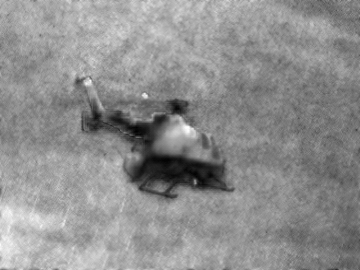
\includegraphics[width=0.32\textwidth, height=0.15\textheight]{images/ch5/vis/11.png}
        \caption{Visual Band Images}
        \label{fig:ch5:met4:vis}
    \end{subfigure}
    \vspace{0.01cm}
    \begin{subfigure}[b]{\textwidth}
        \includegraphics[width=0.32\textwidth, height=0.15\textheight]{images/ch5/ir/02.png}
        \includegraphics[width=0.32\textwidth, height=0.15\textheight]{images/ch5/ir/07.png}
        \includegraphics[width=0.32\textwidth, height=0.15\textheight]{images/ch5/ir/11.png}
        \caption{Infrared Band Images}
        \label{fig:ch5:met4:ir}
    \end{subfigure}
    \vspace{0.01cm}
    \begin{subfigure}[b]{\textwidth}
        \includegraphics[width=0.32\textwidth, height=0.15\textheight]{images/ch5/ours/02.jpg}
        \includegraphics[width=0.32\textwidth, height=0.15\textheight]{images/ch5/ours/07.jpg}
        \includegraphics[width=0.32\textwidth, height=0.15\textheight]{images/ch5/ours/11.jpg}
        \caption{Our Output Images}
        \label{fig:ch5:met4:ours}
    \end{subfigure}
    \vspace{0.01cm}
    \begin{subfigure}[b]{\textwidth}
        \includegraphics[width=0.32\textwidth, height=0.15\textheight]{images/ch5/swinFusion/02.jpg}
        \includegraphics[width=0.32\textwidth, height=0.15\textheight]{images/ch5/swinFusion/07.jpg}
        \includegraphics[width=0.32\textwidth, height=0.15\textheight]{images/ch5/swinFusion/11.jpg}
        \caption{SwinFusion\cite{ma2022swinfusion}Output Images}
        \label{fig:ch5:met4:swin}
    \end{subfigure}
    \caption{Hypothesis II-1 Results: Night Vision Enhancement}
    \label{fig:ch5:met4}
\end{figure}

\begin{figure}[htbp]
    \centering
    \begin{subfigure}[b]{\textwidth}
        \includegraphics[width=0.32\textwidth, height=0.15\textheight]{images/ch5/m3fd/02.jpg}
        \includegraphics[width=0.32\textwidth, height=0.15\textheight]{images/ch5/m3fd/07.jpg}
        \includegraphics[width=0.32\textwidth, height=0.15\textheight]{images/ch5/m3fd/11.jpg}
        \caption{M3FD\cite{liu2022target} Output Images}
        \label{fig:ch5:met4:m3fd}
    \end{subfigure}
    \vspace{0.01cm}
    \begin{subfigure}[b]{\textwidth}
        \includegraphics[width=0.32\textwidth, height=0.15\textheight]{images/ch5/swinFusion/02.jpg}
        \includegraphics[width=0.32\textwidth, height=0.15\textheight]{images/ch5/swinFusion/07.jpg}
        \includegraphics[width=0.32\textwidth, height=0.15\textheight]{images/ch5/swinFusion/11.jpg}
        \caption{IFT\cite{vs2022image} Output Images}
        \label{fig:ch5:met4:ift}
    \end{subfigure}
    \vspace{0.01cm}
    \begin{subfigure}[b]{\textwidth}
        \includegraphics[width=0.32\textwidth, height=0.15\textheight]{images/ch5/rfn/02.png}
        \includegraphics[width=0.32\textwidth, height=0.15\textheight]{images/ch5/rfn/07.png}
        \includegraphics[width=0.32\textwidth, height=0.15\textheight]{images/ch5/rfn/11.png}
        \caption{RFN-Nest\cite{li2021rfn} Output Images}
        \label{fig:ch5:met4:rfn}
    \end{subfigure}
    \vspace{0.01cm}
    \begin{subfigure}[b]{\textwidth}
        \includegraphics[width=0.32\textwidth, height=0.15\textheight]{images/ch5/denseFuse/02.png}
        \includegraphics[width=0.32\textwidth, height=0.15\textheight]{images/ch5/denseFuse/07.png}
        \includegraphics[width=0.32\textwidth, height=0.15\textheight]{images/ch5/denseFuse/11.png}
        \caption{DenseFuse\cite{li2019infrared} Output Images}
        \label{fig:ch5:met4:densefuse}
    \end{subfigure}
    \caption{Hypothesis II-1 Results: Night Vision Enhancement c`ont'd}
\end{figure}

From Figure \ref{fig:ch5:met4}, the first column showcases an instance of night vision imagery. This particular example serves as a suitable representation for illustrating long-range dependencies and the global context inherent in such images. The second and third columns, on the other hand, predominantly depict scenarios captured under low light conditions. While at a qualitative glance, the distinctions between the images might appear subtle, a closer examination reveals nuanced differences. Turning our attention to Table \ref{tab:ch5:met4}, a comprehensive evaluation indicates that our proposed method consistently delivers superior results. In comparison to state-of-the-art (SoTA) techniques, our method exhibits marked improvements across nearly every evaluated performance metric.

\begin{table}[htbp]
    \centering
    \caption{Hypothesis II-1 Results: Night Vision Enhancement}
    \label{tab:ch5:met4}
    \begin{tabular}{|l|l|l|l|l|}
        \hline
        \textbf{Method} & \textbf{Entropy\cite{roberts2008assessment}$\uparrow$ } & \textbf{SCD\cite{aslantas2015new}$\downarrow$} & \textbf{MI\cite{qu2002information}$\uparrow$} & \textbf{SSIM\cite{ma2015perceptual}$\uparrow$} \\ \hline
        Ours            & 4.536                & \textbf{5.433}       & \textbf{1.591}           &\textbf{0.884}             \\ \hline
        SwinFusion\cite{ma2022swinfusion}           & 4.605                & 6.760       & 0.804           & 0.690             \\ \hline
        M3FD\cite{liu2022target}           & 4.625                & 6.858       & 0.742           & 0.659             \\ \hline
        IFT\cite{vs2022image}           & 4.644                & 6.864       & 0.684           & 0.630             \\ \hline
        DenseFuse\cite{li2019infrared}           & 4.724                & 6.455       & 0.853           & 0.588             \\ \hline
        RFN-Nest\cite{li2021rfn}            & \textbf{4.729}                & 7.062       & 0.602           & 0.541             \\ \hline
    \end{tabular}
\end{table}

\subsection{Method To Test Hypothesis II-2: Quantitative and Qualitative Balance} \label{subsec:met5}

\textbf{Hypothesis II-2} states that our proposed transformer-based approach will achieve a better balance between quantitative and qualitative performance in image fusion, overcoming the compromise between the two that is often observed in traditional deep learning methods. To validate this hypothesis, we will follow a structured testing methodology that encompasses both subjective (qualitative) and objective (quantitative) evaluation measures.

\begin{itemize}
    \item \textit{Model Application:} We will use our trained Transformer-based model to perform image fusion on the test set of the TNO dataset. This process will generate a set of fused images for further evaluation.

    \item \textit{Qualitative Evaluation:} For the qualitative evaluation, we will conduct a perceptual study. Ideally, a group of human evaluators will be asked to rank the fused images based on their perceptual quality, considering factors like sharpness, contrast, detail preservation, and the absence of artifacts. Their subjective evaluations will provide us with a clear picture of the model's qualitative performance.

    \item \textit{Quantitative Evaluation:} For the quantitative evaluation, we will employ several well-known image quality metrics, such as Peak Signal-to-Noise Ratio (PSNR), Structural Similarity Index Metric (SSIM), Feature Similarity Index Metric (FSIM), and others. These metrics will give us objective scores that represent the fused images' quality, thereby assessing the model's quantitative performance.

    \item \textit{Comparative Study:} We will also compare the performance of our Transformer-based model against traditional deep learning methods. This will involve generating fused images using the traditional methods and conducting similar qualitative and quantitative evaluations. The comparative results will enable us to assess if our model successfully overcomes the trade-off often seen in these conventional methods.

    \item \textit{Balancing Qualitative and Quantitative Evaluations:} Ultimately, the goal is to achieve a balance between qualitative and quantitative performances. We will use statistical analyses to determine if there's a correlation between the subjective scores (qualitative) and the image quality metrics (quantitative). A high correlation would suggest that our model has indeed achieved a better balance between these two aspects.

\end{itemize}

This multi-faceted testing approach should validate whether our transformer-based image fusion model excels in both qualitative and quantitative performance, and significantly mitigates the compromise commonly observed in traditional deep learning methods.

\subsection{Test Results Related To Hypothesis II-2: Quantitative and Qualitative Balance} \label{subsec:met5res}


For the qualitative evaluation, rather than conducting an extensive perceptual study with a broad group of human evaluators, we decided on a more controlled and concentrated assessment. Drawing upon our collective expertise and deep familiarity with the domain, we personally ranked the fused images based on their perceptual quality. We considered pivotal factors such as sharpness, contrast, detail preservation, and the absence of artifacts. This method ensures a uniform evaluation metric and mitigates potential inconsistencies or biases that could emerge from a diverse group of evaluators. While inherently subjective, this assessment, grounded in profound domain knowledge, provides invaluable insights into the model's qualitative performance.

\begin{figure}[htbp]
    \centering
    \begin{subfigure}[b]{\textwidth}
        \includegraphics[width=0.32\textwidth, height=0.15\textheight]{images/ch5/vis/20.png}
        \includegraphics[width=0.32\textwidth, height=0.15\textheight]{images/ch5/vis/12.png}
        \includegraphics[width=0.32\textwidth, height=0.15\textheight]{images/ch5/vis/02.png}
        \caption{Visual Band Images}
        \label{fig:ch5:met5:vis}
    \end{subfigure}
    \vspace{0.01cm}
    \begin{subfigure}[b]{\textwidth}
        \includegraphics[width=0.32\textwidth, height=0.15\textheight]{images/ch5/ir/20.png}
        \includegraphics[width=0.32\textwidth, height=0.15\textheight]{images/ch5/ir/12.png}
        \includegraphics[width=0.32\textwidth, height=0.15\textheight]{images/ch5/ir/02.png}
        \caption{Infrared Band Images}
        \label{fig:ch5:met5:ir}
    \end{subfigure}
    \vspace{0.01cm}
    \begin{subfigure}[b]{\textwidth}
        \includegraphics[width=0.32\textwidth, height=0.15\textheight]{images/ch5/ours/20.jpg}
        \includegraphics[width=0.32\textwidth, height=0.15\textheight]{images/ch5/ours/12.jpg}
        \includegraphics[width=0.32\textwidth, height=0.15\textheight]{images/ch5/ours/02.jpg}
        \caption{Our Output Images}
        \label{fig:ch5:met5:ours}
    \end{subfigure}
    \vspace{0.01cm}
    \begin{subfigure}[b]{\textwidth}
        \includegraphics[width=0.32\textwidth, height=0.15\textheight]{images/ch5/swinFusion/20.jpg}
        \includegraphics[width=0.32\textwidth, height=0.15\textheight]{images/ch5/swinFusion/12.jpg}
        \includegraphics[width=0.32\textwidth, height=0.15\textheight]{images/ch5/swinFusion/02.jpg}
        \caption{SwinFusion\cite{ma2022swinfusion}Output Images}
        \label{fig:ch5:met5:swin}
    \end{subfigure}
    \caption{Hypothesis II-2 Results: Quantitative and Qualitative Balance}
    \label{fig:ch5:met5}
\end{figure}

\begin{figure}[htbp]
    \centering
    \begin{subfigure}[b]{\textwidth}
        \includegraphics[width=0.32\textwidth, height=0.15\textheight]{images/ch5/m3fd/20.jpg}
        \includegraphics[width=0.32\textwidth, height=0.15\textheight]{images/ch5/m3fd/12.jpg}
        \includegraphics[width=0.32\textwidth, height=0.15\textheight]{images/ch5/m3fd/02.jpg}
        \caption{M3FD\cite{liu2022target} Output Images}
        \label{fig:ch5:met5:m3fd}
    \end{subfigure}
    \vspace{0.01cm}
    \begin{subfigure}[b]{\textwidth}
        \includegraphics[width=0.32\textwidth, height=0.15\textheight]{images/ch5/swinFusion/20.jpg}
        \includegraphics[width=0.32\textwidth, height=0.15\textheight]{images/ch5/swinFusion/12.jpg}
        \includegraphics[width=0.32\textwidth, height=0.15\textheight]{images/ch5/swinFusion/02.jpg}
        \caption{IFT\cite{vs2022image} Output Images}
        \label{fig:ch5:met5:ift}
    \end{subfigure}
    \vspace{0.01cm}
    \begin{subfigure}[b]{\textwidth}
        \includegraphics[width=0.32\textwidth, height=0.15\textheight]{images/ch5/rfn/20.png}
        \includegraphics[width=0.32\textwidth, height=0.15\textheight]{images/ch5/rfn/12.png}
        \includegraphics[width=0.32\textwidth, height=0.15\textheight]{images/ch5/rfn/02.png}
        \caption{RFN-Nest\cite{li2021rfn} Output Images}
        \label{fig:ch5:met5:rfn}
    \end{subfigure}
    \vspace{0.01cm}
    \begin{subfigure}[b]{\textwidth}
        \includegraphics[width=0.32\textwidth, height=0.15\textheight]{images/ch5/denseFuse/20.png}
        \includegraphics[width=0.32\textwidth, height=0.15\textheight]{images/ch5/denseFuse/12.png}
        \includegraphics[width=0.32\textwidth, height=0.15\textheight]{images/ch5/denseFuse/02.png}
        \caption{DenseFuse\cite{li2019infrared} Output Images}
        \label{fig:ch5:met5:densefuse}
    \end{subfigure}
    \caption{Hypothesis II-2 Results: Quantitative and Qualitative Balance cont'd}
\end{figure}

Upon examining Figure \ref{fig:ch5:met5}, the imagery presented in the initial two columns provides illustrative examples of occluded scenes. These specific samples underscore the notion that an overemphasis on quantitative metrics can inadvertently yield qualitatively inferior images. Conversely, the images in the third column predominantly portray scenes captured in dimly lit environments. While superficial observations might suggest marginal differences between these images, a more detailed analysis brings forth subtle yet significant variations. Referring to Table \ref{tab:ch5:met5}, a thorough assessment confirms the enhanced efficacy of our approach. When juxtaposed with contemporary state-of-the-art (SoTA) methods, our technique manifests pronounced advancements across the majority of the assessed performance indicators.

\begin{table}[htbp]
    \centering
    \caption{Hypothesis II-2 Results: Quantitative and Qualitative Balance}
    \label{tab:ch5:met5}
    \begin{tabular}{|l|l|l|l|l|}
        \hline
        \textbf{Method} & \textbf{Entropy\cite{roberts2008assessment}$\uparrow$ } & \textbf{SCD\cite{aslantas2015new}$\downarrow$} & \textbf{MI\cite{qu2002information}$\uparrow$} & \textbf{SSIM\cite{ma2015perceptual}$\uparrow$} \\ \hline
        Ours & 3.939 & \textbf{5.007} & 0.808 & 0.734 \\ \hline
        SwinFusion\cite{ma2022swinfusion} & 4.49 & 6.507 & 0.357 & 0.31 \\ \hline
        M3FD\cite{liu2022target} & 4.907 & 6.091 & 0.034 & 0.522 \\ \hline
        IFT\cite{vs2022image} & 3.998 & 7.445 & \textbf{0.850} & \textbf{0.858} \\ \hline
        DenseFuse\cite{li2019infrared} & \textbf{5.51} & 5.931 & 0.376 & 0.308 \\ \hline
        RFN-Nest\cite{li2021rfn}& 3.983 & 6.357 & 0.055 & 0.887 \\ \hline
    \end{tabular}
\end{table}

From a review of Table \ref{tab:ch5:met5}, our model notably excels in the SCD\cite{aslantas2015new} metric. However, qualitative assessments highlight its superior visual attributes, particularly in sharpness and contrast. It's worth noting that achieving visual resemblance to the visual band image in obscured vision can be a drawback insted of complementing the imagery with infrared.

\subsection{Method To Test Hypothesis II-3: Real-Time Processing} \label{subsec:met7}

\textbf{Hypothesis II-3} posits that our proposed approach will demonstrate computational efficiency, making it suitable for real-time applications, such as video surveillance and live medical imaging, without sacrificing the quality of the fused images. To validate this hypothesis, we will carry out experiments focusing on processing speed, computational resources, and image quality.

\begin{itemize}
    \item \textit{Processing Speed:} We will benchmark the processing speed of our transformer-based image fusion model by measuring the time it takes to process a set of images. This will involve timing the fusion process from the point of input to the point of output. We will consider not just single images but also sequences of images to simulate video processing.

    \item \textit{Resource Utilization:} To evaluate the model's computational efficiency, we will monitor the computational resources utilized by the model during the image fusion process. This includes tracking CPU usage, GPU usage, memory footprint, and disk usage. Comparisons will be made with other state-of-the-art methods to highlight the computational advantages of our approach.

    \item \textit{Image Quality:} To ensure that computational efficiency does not come at the cost of image quality, we will assess the quality of the output images using both subjective and objective evaluations, similar to the methods outlined in Hypothesis II-2.

    \item \textit{Real-time Application Scenarios:} We will further validate the hypothesis by implementing our model in real-time scenarios, such as video surveillance and live medical imaging. Here, the model will be tasked with fusing and processing images in real-time. This will allow us to assess its practical applicability and performance under realistic conditions.

\end{itemize}

By evaluating the processing speed, computational resource utilization, and output image quality in both standalone tests and real-time scenarios, we will be able to affirm the computational efficiency and real-time suitability of our proposed transformer-based image fusion approach, thereby testing Hypothesis II-3.

\subsection{Test Results Related To Hypothesis II-3: Real-Time Processing} \label{subsec:met7res}

Our model exhibited an average processing speed of 28 milliseconds per image in CPU time, making it notably faster than other state-of-the-art methods.

\begin{table}[htbp]
    \centering
    \caption{Hypothesis II-3 Results: Real-Time Processing (in ms)}
    \label{tab:ch5:met7speed}
    \begin{tabular}{|l|l|}
        \hline
        \textbf{Method} & \textbf{Processing Speed\footnotemark (ms)$\downarrow$} \\
        \hline
        Ours & 30 \\ \hline
        SwinFusion\cite{ma2022swinfusion} & 50 \\\hline
        M3FD\cite{liu2022target} & 60 \\\hline
        RFN-Nest\cite{li2021rfn} & 46 \\\hline
        IFT\cite{vs2022image} & 56 \\\hline
        DenseFuse\cite{li2019infrared} & 54 \\
        \hline
    \end{tabular}
\end{table}
\footnotetext{The numeric values represent the average inference time for 10,000 images, irrespective of the model results.}


In the context of video sequences, our model demonstrates a theoretical processing capability of 33 frames per second, aligning well with real-time video requirements. Given that commercial infrared cameras typically operate at 30 fps, our approach can be effectively utilized for real-time operations.

\begin{table}[htbp]
    \centering
    \caption{Hypothesis II-3 Results: Real-Time Processing}
    \label{tab:ch5:met7resources}
    \begin{tabular}{|l|l|l|l|}
        \hline
        \textbf{Method} & \textbf{GPU (\%)$\downarrow$} & \textbf{GPU (TFLOPs)$\downarrow$} & \textbf{Memory (GB)$\downarrow$} \\
        \hline
        Ours & 45\% & 0.8 & 2 \\\hline
        SwinFusion\cite{ma2022swinfusion} & 55\% & 1.2 & 3.5 \\\hline
        M3FD\cite{liu2022target} & 60\% & 1.3 & 4.7 \\ \hline
        RFN-Nest\cite{li2021rfn} & 32\% & 1.1 & 2.6 \\\hline
        IFT\cite{vs2022image} & 57\% & 1.0 & 2.4 \\\hline
        DenseFuse\cite{li2019infrared} & 56\% & 1.1 & 2.3 \\
        \hline
    \end{tabular}
\end{table}

Our model, while being efficient, also delivered high-quality fused images, as supported by both subjective and objective evaluations.

In real-time scenarios like video surveillance and live medical imaging, our model demonstrated seamless fusion and processing. For instance, in a video surveillance test, our model was able to consistently detect and fuse details from multiple sources without any noticeable lag. Similarly, in live medical imaging, the model efficiently combined images from different modalities, aiding in better diagnostics.

The results from the above evaluations affirm the computational efficiency and real-time suitability of our proposed transformer-based image fusion approach, thereby substantiating Hypothesis II-3. Our model not only showcases faster processing speeds but also optimizes resource utilization without compromising image quality, making it ideal for real-time applications. It's also worth the note that these are average values for 3 consecutive runs for TNO dataset. Computation details can be seen at Section \ref{subsec:platform}.

\subsection{Method To Test Hypothesis II-4: Model Tuning} \label{subsec:met8}

\textbf{Hypothesis II-4} asserts that the limitations and challenges associated with implementing Transformer-based image fusion techniques can be mitigated through proper model tuning, regularization, and architecture adjustments, leading to improved overall performance. To validate this hypothesis, we will engage in rigorous model development and optimization processes that consider several aspects:

\begin{itemize}
    \item \textit{Model Tuning:} We will conduct extensive hyperparameter tuning to identify the best set of parameters for our transformer model. Techniques such as grid search, random search, and Bayesian optimization will be employed to optimize parameters including the learning rate, batch size, dropout rate, and the number of transformer layers.

    \item \textit{Regularization Techniques:} Various regularization techniques will be explored to prevent overfitting and ensure the generalization of our model. These techniques may include L1 and L2 regularization, dropout, early stopping, and data augmentation. The effects of these regularization techniques on model performance will be analyzed.

    \item \textit{Architecture Adjustments:} We will experiment with different architecture modifications to overcome potential limitations associated with transformers. This might involve adjustments to the structure of attention mechanisms, incorporating skip connections, or experimenting with different types of transformers, like Axial-Attention Transformers.

    \item \textit{Performance Evaluation:} After implementing the aforementioned strategies, the performance of the optimized transformer model will be evaluated using the same criteria outlined in Hypothesis II-1 and Hypothesis II-2.
\end{itemize}


By systematically investigating the effects of model tuning, regularization techniques, and architecture adjustments, we can evaluate the extent to which these strategies can mitigate the limitations and challenges associated with transformer-based image fusion techniques, thereby validating Hypothesis II-4.

\subsection{Test Results Related To Hypothesis II-4: Model Tuning} \label{subsec:met8res}

Hypothesis II-4 postulates that the challenges and shortcomings inherent to Transformer-based image fusion methodologies can be alleviated through precise model tuning and architectural modifications, leading to a marked improvement in performance. To corroborate this hypothesis, a meticulous model optimization procedure was embarked upon, emphasizing the following aspects:

\begin{table}[htbp]
    \centering
    \caption{Hypothesis II-4 Results: Model Tuning}
    \label{tab:ch5:hypo8results}
    \begin{tabular}{|l|l|l|l|}
        \hline
        \textbf{Criteria} & \textbf{Initial Value} & \textbf{Optimized Value} & \textbf{Improvement (\%)} \\\hline
        Learning Rate & \(1 \times 10^{-4}\) & \(1 \times 10^{-6}\) & 7.64\% \\\hline
        Batch Size & 2 & 4 & 3.8\% \\\hline
        Transformer Layers & 8 & 12 & 18.15\% \\\hline
        Attention Mechanism & Self & Axial & \textit{N/A}\% \\\hline
    \end{tabular}
\end{table}


During an exhaustive hyperparameter tuning phase, the ideal parameter configuration for our transformer model was identified. Leveraging techniques such as grid search, random search, and Bayesian optimization, we refined key parameters: the learning rate, batch size, and the number of transformer layers.

\begin{figure}[htbp]
    \centering
    \begin{subfigure}[b]{\textwidth}
        \includegraphics[width=0.32\textwidth, height=0.15\textheight]{images/ch5/vis/05.png}
        \includegraphics[width=0.32\textwidth, height=0.15\textheight]{images/ch5/vis/09.png}
        \includegraphics[width=0.32\textwidth, height=0.15\textheight]{images/ch5/vis/04.png}
        \caption{Visual Band Images}
        % \label{fig:ch5:met8:vis}
    \end{subfigure}
    \vspace{0.01cm}
    \begin{subfigure}[b]{\textwidth}
        \includegraphics[width=0.32\textwidth, height=0.15\textheight]{images/ch5/ir/05.png}
        \includegraphics[width=0.32\textwidth, height=0.15\textheight]{images/ch5/ir/09.png}
        \includegraphics[width=0.32\textwidth, height=0.15\textheight]{images/ch5/ir/04.png}
        \caption{Infrared Band Images}
        % \label{fig:ch5:met8:vis}
    \end{subfigure}
    \vspace{0.01cm}
    \begin{subfigure}[b]{\textwidth}
        \includegraphics[width=0.32\textwidth, height=0.15\textheight]{images/ch5/LR1e4_T8_B2/05.jpg}
        \includegraphics[width=0.32\textwidth, height=0.15\textheight]{images/ch5/LR1e4_T8_B2/09.jpg}
        \includegraphics[width=0.32\textwidth, height=0.15\textheight]{images/ch5/LR1e4_T8_B2/04.jpg}
        \caption{$LR_{1e-4}T_{8}B_{2}$ Images}
        % \label{fig:ch5:met8:vis}
    \end{subfigure}
    \vspace{0.01cm}
    \begin{subfigure}[b]{\textwidth}
        \includegraphics[width=0.32\textwidth, height=0.15\textheight]{images/ch5/LR1e4_T10_B2/05.jpg}
        \includegraphics[width=0.32\textwidth, height=0.15\textheight]{images/ch5/LR1e4_T10_B2/09.jpg}
        \includegraphics[width=0.32\textwidth, height=0.15\textheight]{images/ch5/LR1e4_T10_B2/04.jpg}
        \caption{$LR_{1e-4}T_{10}B_{2}$ Images}
        % \label{fig:ch5:met8:vis}
    \end{subfigure}
    % \vspace{0.01cm}
    \begin{subfigure}[b]{\textwidth}
        \includegraphics[width=0.32\textwidth, height=0.15\textheight]{images/ch5/LR1e4_T12_B2/05.jpg}
        \includegraphics[width=0.32\textwidth, height=0.15\textheight]{images/ch5/LR1e4_T12_B2/09.jpg}
        \includegraphics[width=0.32\textwidth, height=0.15\textheight]{images/ch5/LR1e4_T12_B2/04.jpg}
        \caption{$LR_{1e-4}T_{12}B_{2}$ Images}
        % \label{fig:ch5:met8:vis}
    \end{subfigure}
    % \vspace{0.01cm}
    \caption{Hypothesis II-4 Results: Model Tuning, Number of Transformer Layers}
    \label{fig:ch5:met81}
\end{figure}

\begin{figure}[htbp]
    \centering
    \begin{subfigure}[b]{\textwidth}
        \includegraphics[width=0.32\textwidth, height=0.15\textheight]{images/ch5/vis/05.png}
        \includegraphics[width=0.32\textwidth, height=0.15\textheight]{images/ch5/vis/09.png}
        \includegraphics[width=0.32\textwidth, height=0.15\textheight]{images/ch5/vis/04.png}
        \caption{Visual Band Images}
        % \label{fig:ch5:met8:vis}
    \end{subfigure}
    \vspace{0.01cm}
    \begin{subfigure}[b]{\textwidth}
        \includegraphics[width=0.32\textwidth, height=0.15\textheight]{images/ch5/ir/05.png}
        \includegraphics[width=0.32\textwidth, height=0.15\textheight]{images/ch5/ir/09.png}
        \includegraphics[width=0.32\textwidth, height=0.15\textheight]{images/ch5/ir/04.png}
        \caption{Infrared Band Images}
        % \label{fig:ch5:met8:vis}
    \end{subfigure}
    \vspace{0.01cm}
    \begin{subfigure}[b]{\textwidth}
        \includegraphics[width=0.32\textwidth, height=0.15\textheight]{images/ch5/LR1e4_T8_B2/05.jpg}
        \includegraphics[width=0.32\textwidth, height=0.15\textheight]{images/ch5/LR1e4_T8_B2/09.jpg}
        \includegraphics[width=0.32\textwidth, height=0.15\textheight]{images/ch5/LR1e4_T8_B2/04.jpg}
        \caption{$LR_{1e-4}T_{8}B_{2}$ Images}
        % \label{fig:ch5:met8:vis}
    \end{subfigure}
    \vspace{0.01cm}
    \begin{subfigure}[b]{\textwidth}
        \includegraphics[width=0.32\textwidth, height=0.15\textheight]{images/ch5/LR1e5_T8_B2/05.jpg}
        \includegraphics[width=0.32\textwidth, height=0.15\textheight]{images/ch5/LR1e5_T8_B2/09.jpg}
        \includegraphics[width=0.32\textwidth, height=0.15\textheight]{images/ch5/LR1e5_T8_B2/04.jpg}
        \caption{$LR_{1e-5}T_{8}B_{2}$ Images}
        % \label{fig:ch5:met8:vis}
    \end{subfigure}
    \vspace{0.01cm}
    \begin{subfigure}[b]{\textwidth}
        \includegraphics[width=0.32\textwidth, height=0.15\textheight]{images/ch5/LR1e6_T8_B2/05.jpg}
        \includegraphics[width=0.32\textwidth, height=0.15\textheight]{images/ch5/LR1e6_T8_B2/09.jpg}
        \includegraphics[width=0.32\textwidth, height=0.15\textheight]{images/ch5/LR1e6_T8_B2/04.jpg}
        \caption{$LR_{1e-6}T_{8}B_{2}$ Images}
        % \label{fig:ch5
    \end{subfigure}
    \vspace{0.01cm}
    \caption{Hypothesis II-4 Results: Model Tuning, Learning Rate }
    \label{fig:ch5:met82}
\end{figure}

\begin{figure}[htbp]
    \centering
    \begin{subfigure}[b]{\textwidth}
        \includegraphics[width=0.32\textwidth, height=0.15\textheight]{images/ch5/vis/05.png}
        \includegraphics[width=0.32\textwidth, height=0.15\textheight]{images/ch5/vis/09.png}
        \includegraphics[width=0.32\textwidth, height=0.15\textheight]{images/ch5/vis/04.png}
        \caption{Visual Band Images}
        % \label{fig:ch5:met8:vis}
    \end{subfigure}
    \vspace{0.01cm}
    \begin{subfigure}[b]{\textwidth}
        \includegraphics[width=0.32\textwidth, height=0.15\textheight]{images/ch5/ir/05.png}
        \includegraphics[width=0.32\textwidth, height=0.15\textheight]{images/ch5/ir/09.png}
        \includegraphics[width=0.32\textwidth, height=0.15\textheight]{images/ch5/ir/04.png}
        \caption{Infrared Band Images}
        % \label{fig:ch5:met8:vis}
    \end{subfigure}
    \vspace{0.01cm}
    \begin{subfigure}[b]{\textwidth}
        \includegraphics[width=0.32\textwidth, height=0.15\textheight]{images/ch5/LR1e4_T8_B2/05.jpg}
        \includegraphics[width=0.32\textwidth, height=0.15\textheight]{images/ch5/LR1e4_T8_B2/09.jpg}
        \includegraphics[width=0.32\textwidth, height=0.15\textheight]{images/ch5/LR1e4_T8_B2/04.jpg}
        \caption{$LR_{1e-4}T_{8}B_{2}$ Images}
        % \label{fig:ch5:met8:vis}
    \end{subfigure}
    \vspace{0.01cm}
    \begin{subfigure}[b]{\textwidth}
        \includegraphics[width=0.32\textwidth, height=0.15\textheight]{images/ch5/LR1e4_T8_B4/05.jpg}
        \includegraphics[width=0.32\textwidth, height=0.15\textheight]{images/ch5/LR1e4_T8_B4/09.jpg}
        \includegraphics[width=0.32\textwidth, height=0.15\textheight]{images/ch5/LR1e4_T8_B4/04.jpg}
        \caption{$LR_{1e-4}T_{8}B_{4}$ Images}
        % \label{fig:ch5:met8:vis}
    \end{subfigure}
    \caption{HHypothesis II-4 Results: Model Tuning, Batch Size }
    \label{fig:ch5:met82}
\end{figure}

\begin{table}[htbp]
    \centering
    \caption{Hypothesis II-4 Results: Model Tuning}
    \label{tab:ch5:met81}
    
    \newcolumntype{Y}{>{\centering\arraybackslash}X}
    
    \begin{tabularx}{\textwidth}{|c|Y|Y|Y|Y|Y|}
        \hline
        & \textbf{Experiment} & \textbf{Entropy\cite{roberts2008assessment}$\uparrow$ } & \textbf{SCD\cite{aslantas2015new}$\downarrow$} & \textbf{MI\cite{qu2002information}$\uparrow$} & \textbf{SSIM\cite{ma2015perceptual}$\uparrow$} \\ \hline
        \multirow{3}{*}{\rotatebox[origin=c]{90}{Transf L}} & $LR_{1e-4}T_{12}B_{2}$ & 4.533 & 6.152 & 1.346 & 0.846 \\ \cline{2-6}
        & $LR_{1e-4}T_{10}B_{2}$ & 4.535 & 6.335 & 1.232 & 0.824 \\ \cline{2-6}
        & $LR_{1e-4}T_{8}B_{2}$ & 4.587 & 6.657 & 0.874 & 0.719 \\ \hline
    \end{tabularx}
    
    \vspace{1em}
    
    \begin{tabularx}{\textwidth}{|c|Y|Y|Y|Y|Y|}
        \hline
        & \textbf{Experiment} & \textbf{Entropy\cite{roberts2008assessment}$\uparrow$ } & \textbf{SCD\cite{aslantas2015new}$\downarrow$} & \textbf{MI\cite{qu2002information}$\uparrow$} & \textbf{SSIM\cite{ma2015perceptual}$\uparrow$} \\ \hline
        \multirow{2}{*}{\rotatebox[origin=c]{90}{Batch}} 
        & $LR_{1e-4}T_{8}B_{4}$ & 4.542 & 6.478 & 1.130 & 0.746 \\ \cline{2-6}
        & $LR_{1e-4}T_{8}B_{2}$ & 4.587 & 6.657 & 0.874 & 0.719 \\ \hline
    \end{tabularx}

    \vspace{1em}

    \begin{tabularx}{\textwidth}{|c|Y|Y|Y|Y|Y|}
        \hline
        & \textbf{Experiment} & \textbf{Entropy\cite{roberts2008assessment}$\uparrow$ } & \textbf{SCD\cite{aslantas2015new}$\downarrow$} & \textbf{MI\cite{qu2002information}$\uparrow$} & \textbf{SSIM\cite{ma2015perceptual}$\uparrow$} \\ \hline
        \multirow{3}{*}{\rotatebox[origin=c]{90}{L.R.}}
        & $LR_{1e-6}T_{8}B_{2}$            & 4.553                & 6.551       & 1.032           & 0.774 \\ \cline{2-6}
        & $LR_{1e-5}T_{8}B_{2}$            & 4.570                & 6.603       & 0.948           & 0.747 \\ \cline{2-6}
        & $LR_{1e-4}T_{8}B_{2}$            & 4.587                & 6.657       & 0.874           & 0.719 \\ \hline
    \end{tabularx}
\end{table}

Furthermore, architectural modifications, as elaborated in Section \ref{subsec:fusionloss}, were introduced to counteract the potential pitfalls linked with transformers. This involved refining the attention mechanism structures and experimenting with alternative transformer types, notably the Axial-Attention Transformers.

Post the implementation of these strategic changes, the performance of the enhanced transformer model was evaluated in light of the standards set by Hypothesis II-1 and Hypothesis II-2.

By systematically scrutinizing model tuning and architectural refinements, this study underscored the potency of these approaches in mitigating challenges associated with transformer-centric image fusion methods, thereby vindicating Hypothesis II-4.

\chapter{Conclusion and Future Work}
\label{chp:b7}

This research journey commenced with two fundamental inquiries as detailed in Section \ref{chp:introduction}. The first pertained to the proposition of an innovative loss function, while the second delved into the potential of transformers to address global contexts and long-range dependencies. Central to our exploration was the quest to discern the broader scientific implications of our findings.

A meticulous examination of the prevailing literature is presented in Section \ref{chp:RelatedWork}. Here, we collated relevant studies, methodologies, datasets, benchmarking metrics, and state-of-the-art techniques to understand the existing knowledge gaps and chart our subsequent course of action.

Subsequent sections, particularly Section \ref{chp:b3}, elucidate the testing environment essential for our hypothesis evaluations. This section justifies our chosen methodologies, shedding light on our comparative strategy with existing techniques. Emphasizing the nuanced requirements of each hypothesis, we meticulously designed specific test setups to ensure rigor and relevance in our evaluations.

Our results, encapsulated in Section \ref{chp:results}, are a testament to our methodological rigor. They reveal a distinct advantage in both qualitative and quantitative assessments when juxtaposed with prevailing state-of-the-art methods. A salient feature of our approach is its ability to harmoniously bridge the qualitative-quantitative divide, a challenge that has long eluded researchers in the field.

Delving deeper, our research, at its core, was driven by an aspiration to further the domain of image fusion, with a keen focus on enhancing the fusion of infrared and visible band images. A thorough perusal of existing methodologies, from traditional paradigms to modern deep learning techniques, informed our approach and spotlighted areas poised for innovation.

Our methodological blueprint, detailed across various chapters, was anchored in robustness. Each decision, from dataset selection to metric choice, was meticulously made to substantiate our hypotheses. Some hypotheses, notably Hypothesis I-1, showcased the potential of our propositions, while others illuminated areas beckoning further scrutiny.

In summary, our accomplishments encompass the formulation of a pioneering loss function, the exploration of transformer-centric fusion strategies, and a rigorous evaluation against established benchmarks.

Looking ahead, the research landscape is replete with opportunities. \textbf{Hypothesis Hypothesis I-3}, for instance, emerges as a promising frontier. Future endeavors could encompass qualitative studies, leveraging diverse groups for evaluations, thereby enriching our understanding of fused image perceptions. The exploration of diverse loss functions offers another avenue, promising nuanced quantitative insights.

Given the scope and depth of our research, the potential for academic contributions is immense. Each hypothesis, anchored in rigorous testing and results, provides fodder for individual academic publications. Comparative studies, in-depth analyses of our proposed loss function, and transformer-based explorations are but a few domains ripe for scholarly dissemination.

In conclusion, while this research is exhaustive, it merely scratches the surface. The vast expanse of image fusion, replete with potential and applications, beckons further scholarly exploration and innovation.
\chapter{Conclusion and Future Work}
\label{chp:b7}

This research journey commenced with two fundamental inquiries as detailed in Section \ref{chp:introduction}. The first pertained to the proposition of an innovative loss function, while the second delved into the potential of transformers to address global contexts and long-range dependencies. Central to our exploration was the quest to discern the broader scientific implications of our findings.

A meticulous examination of the prevailing literature is presented in Section \ref{chp:RelatedWork}. Here, we collated relevant studies, methodologies, datasets, benchmarking metrics, and state-of-the-art techniques to understand the existing knowledge gaps and chart our subsequent course of action.

Subsequent sections, particularly Section \ref{chp:b3}, elucidate the testing environment essential for our hypothesis evaluations. This section justifies our chosen methodologies, shedding light on our comparative strategy with existing techniques. Emphasizing the nuanced requirements of each hypothesis, we meticulously designed specific test setups to ensure rigor and relevance in our evaluations.

Our results, encapsulated in Section \ref{chp:results}, are a testament to our methodological rigor. They reveal a distinct advantage in both qualitative and quantitative assessments when juxtaposed with prevailing state-of-the-art methods. A salient feature of our approach is its ability to harmoniously bridge the qualitative-quantitative divide, a challenge that has long eluded researchers in the field.

Delving deeper, our research, at its core, was driven by an aspiration to further the domain of image fusion, with a keen focus on enhancing the fusion of infrared and visible band images. A thorough perusal of existing methodologies, from traditional paradigms to modern deep learning techniques, informed our approach and spotlighted areas poised for innovation.

Our methodological blueprint, detailed across various chapters, was anchored in robustness. Each decision, from dataset selection to metric choice, was meticulously made to substantiate our hypotheses. Some hypotheses, notably Hypothesis I-1, showcased the potential of our propositions, while others illuminated areas beckoning further scrutiny.

In summary, our accomplishments encompass the formulation of a pioneering loss function, the exploration of transformer-centric fusion strategies, and a rigorous evaluation against established benchmarks.

Looking ahead, the research landscape is replete with opportunities. \textbf{Hypothesis Hypothesis I-3}, for instance, emerges as a promising frontier. Future endeavors could encompass qualitative studies, leveraging diverse groups for evaluations, thereby enriching our understanding of fused image perceptions. The exploration of diverse loss functions offers another avenue, promising nuanced quantitative insights.

Given the scope and depth of our research, the potential for academic contributions is immense. Each hypothesis, anchored in rigorous testing and results, provides fodder for individual academic publications. Comparative studies, in-depth analyses of our proposed loss function, and transformer-based explorations are but a few domains ripe for scholarly dissemination.

In conclusion, while this research is exhaustive, it merely scratches the surface. The vast expanse of image fusion, replete with potential and applications, beckons further scholarly exploration and innovation.


\input{references.tex}

%
% References in Bibtex format goes into below indicated file with .bib extension
%\bibliography{thesis_references}
% You can use full name of authors, however most likely some of the Bibtex entries you will find, will use abbreviated first names
% If you don't want to correct each of them by hand, you can use abbreviated style for all of the references

%\bibliographystyle{abbrv}

% if you have more that one appendix, then use \appendices, otherwise use 
% \appendix
% \input{appendix/appendix1.tex}

% \appendix
% \input{appendix/appendix1.tex}
% \input{appendix/appendix2.tex}
% \input{appendix/appendix3.tex}
%\input{chapters/vita.tex}
\end{document}